%\begin{figure}[!t]
%    \centering
%    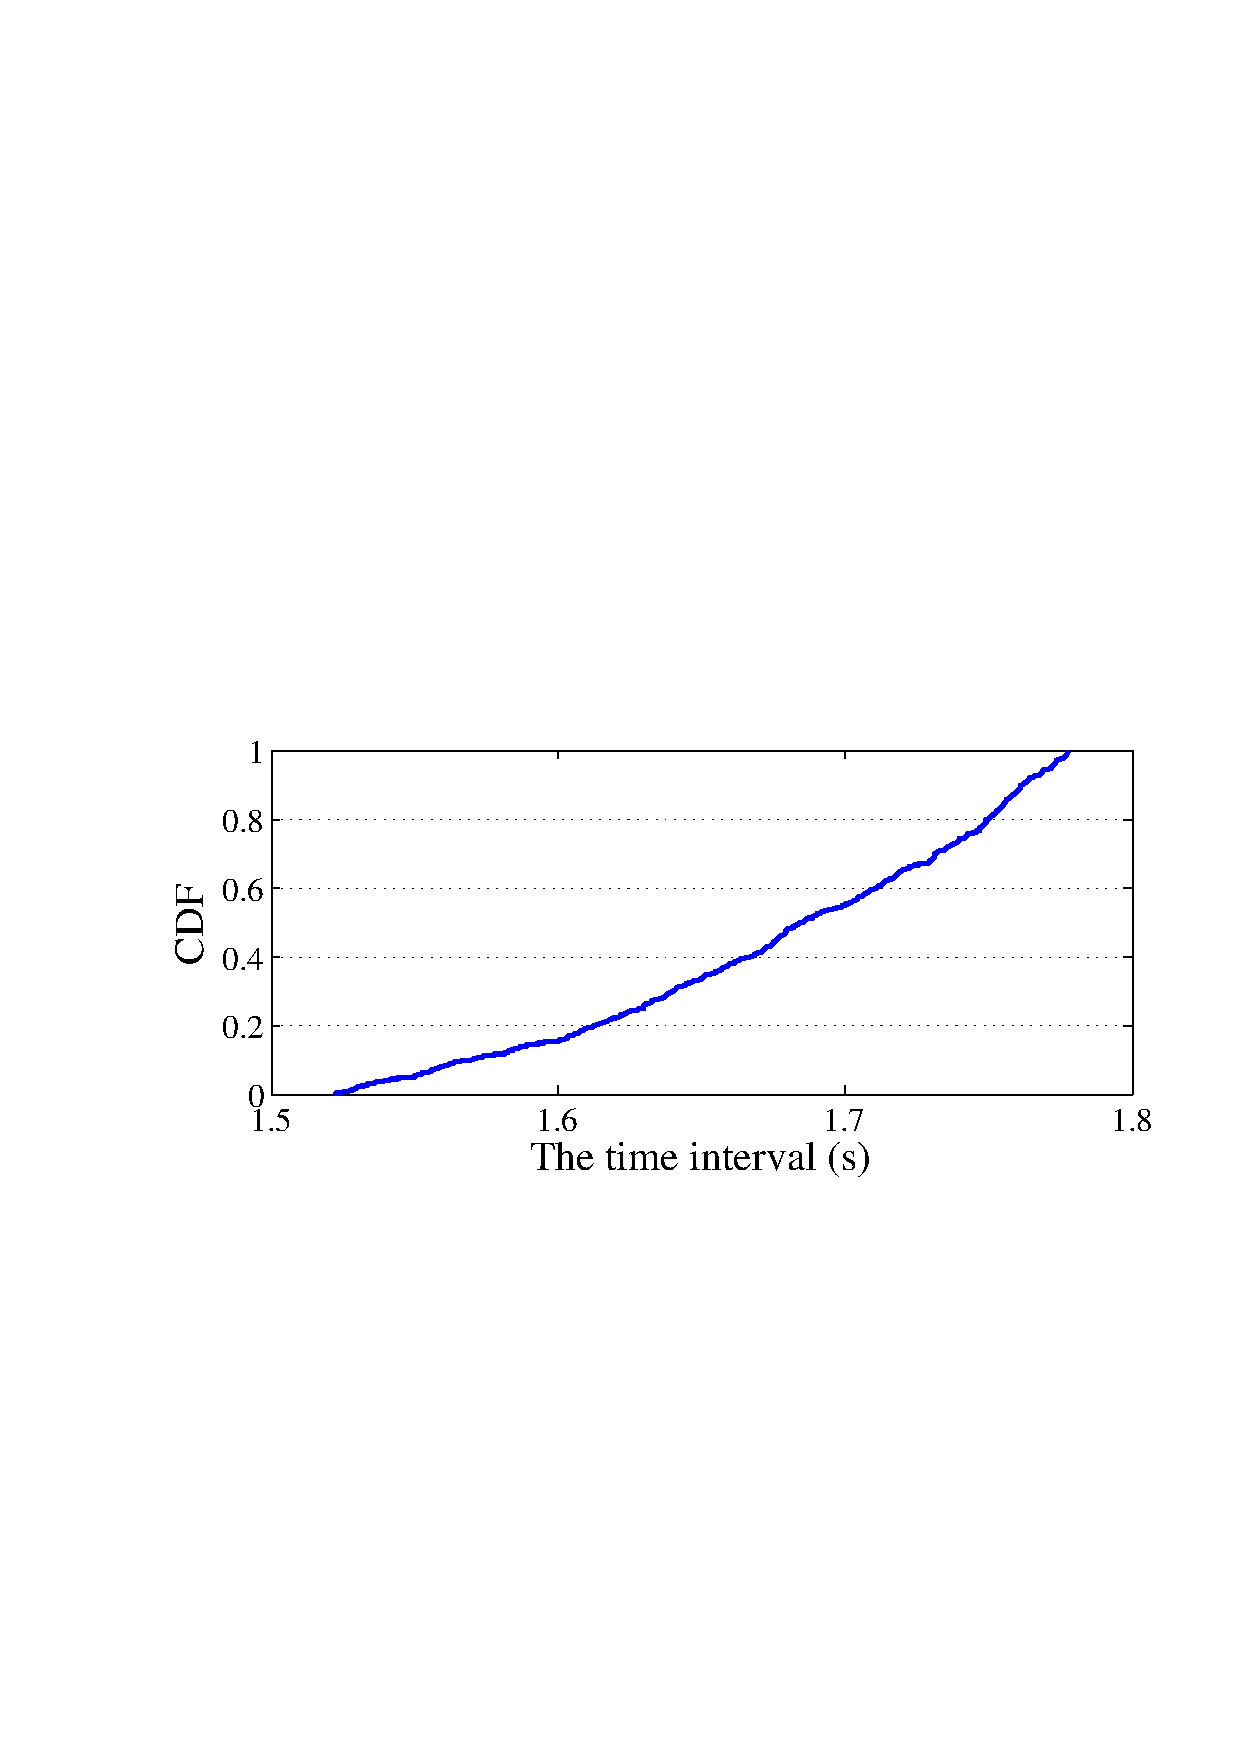
\includegraphics[width=0.45\textwidth]{fig/time-interval.pdf}
%    \caption{The cumulative distribution function (CDF) of the time interval between pattern drawing and other on-screen activities.}
%    \label{fig:time-interval}
%    \vspace{-5mm}
%\end{figure}
\vspace{-2mm}
\section{Implementation Details}

\subsection{Video preprocessing \label{sec:identify}}
\label{section:recognition}
The first step of our attack is to identify the unlocking process from the
video footage. While all our
participants (see Section~\ref{section:locking patterns}) consider this as a straightforward manual task, we developed a \emph{simple yet effective} heuristic to automatically detect the video segment in some typical scenarios. Our heuristic is based on the following observations: (1) before or after
unlocking, users often pause for a few seconds; (2) two consecutive on-screen operations (e.g. swiping, zooming etc.) typically expose some spatial-temporal motion characteristics.

In our initial test, we find that there exists at least $1.5$ seconds pause before or after pattern drawing due to delay of the user or the device. We also found that identical on-screen activities often follow closely. For example, on several occasions our participants had to swipe several times  to locate a program from the application list.
These consecutive on-screen operations have some spatial-temporal motion characteristics that are different from pattern drawing.
Figure~\ref{fig:gesture-distinction} shows the spatial-temporal motion structure for  two gestures, swiping and zooming, when they are performed once (a, c) and twice (b, d).
This diagram indicates that the spatial-temporal motion of two identical on-sreen activities contains one or more looping structures for which pattern drawing does not have.

%In order to test our hypothesis, we have recorded 50 video streams (each
%video lasts around 2 minutes) of how ten of our participants drew
%patterns. During video recording, our participants firstly performed
%some on-screen activities such as web browsing and gaming as they wished;
%they then opened up a pattern lock screen to draw a pattern and
%continued to perform other on-screen operations afterwards.
%For each video stream, we then analyzed frames that are associated with pattern drawing and those are not.
%
%
%Figure~\ref{fig:time-interval} shows that all our participants paused at least $1.5$ seconds before or after pattern drawing due to delay of the user or the device.
%%Our algorithm leverages this characteristic to locate the start and end point of unlocking process.
%We also found that identical on-screen activities often follow closely. For example, on several occasions our participants had to swipe several times  to locate a program from the application list.
%These consecutive on-screen operations have some spatial-temporal motion characteristics that are different from pattern drawing.
%Figure~\ref{fig:gesture-distinction} shows the spatial-temporal motion structure for  two gestures, swiping and zooming, when they are performed once (a, c, e) and twice (b, d, f).
%This diagram indicates that the spatial-temporal motion of two identical on-sreen activities contains one or more looping structures for which pattern drawing does not have.

    \begin{figure}[!t]
        \vspace{-5mm}
        \centering
        \subfigure{
            \begin{minipage}[t]{0.19\textwidth}
            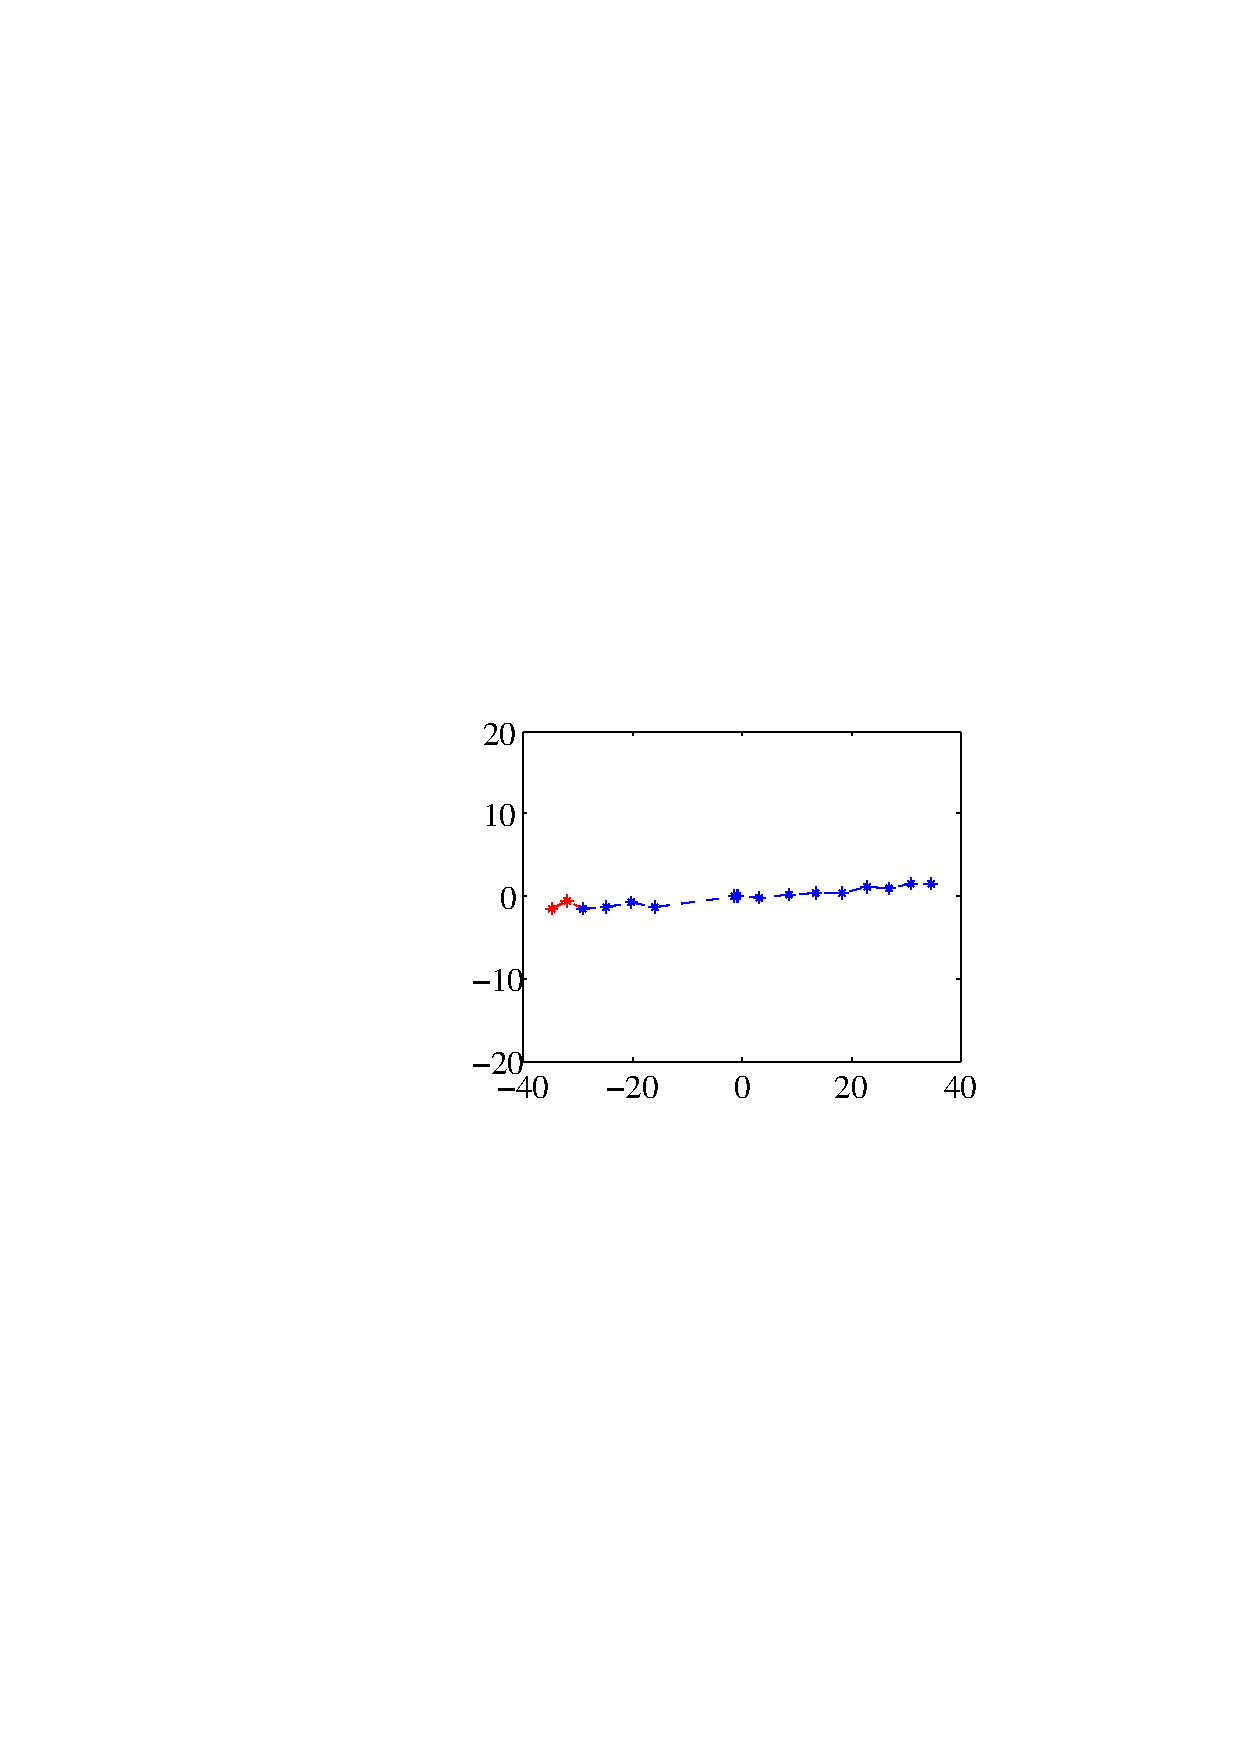
\includegraphics[width=\textwidth]{fig/gesture-distinction1.pdf}\\
            \centering  (a) a horizontal-swiping gesture
            %\FIXME{Need to mark the starting point and turning point}
            \end{minipage}
        }
        \vspace{-3mm}
        \hspace{0.25cm}
        %\hfill
        \subfigure{
            \begin{minipage}[t]{0.19\textwidth}
            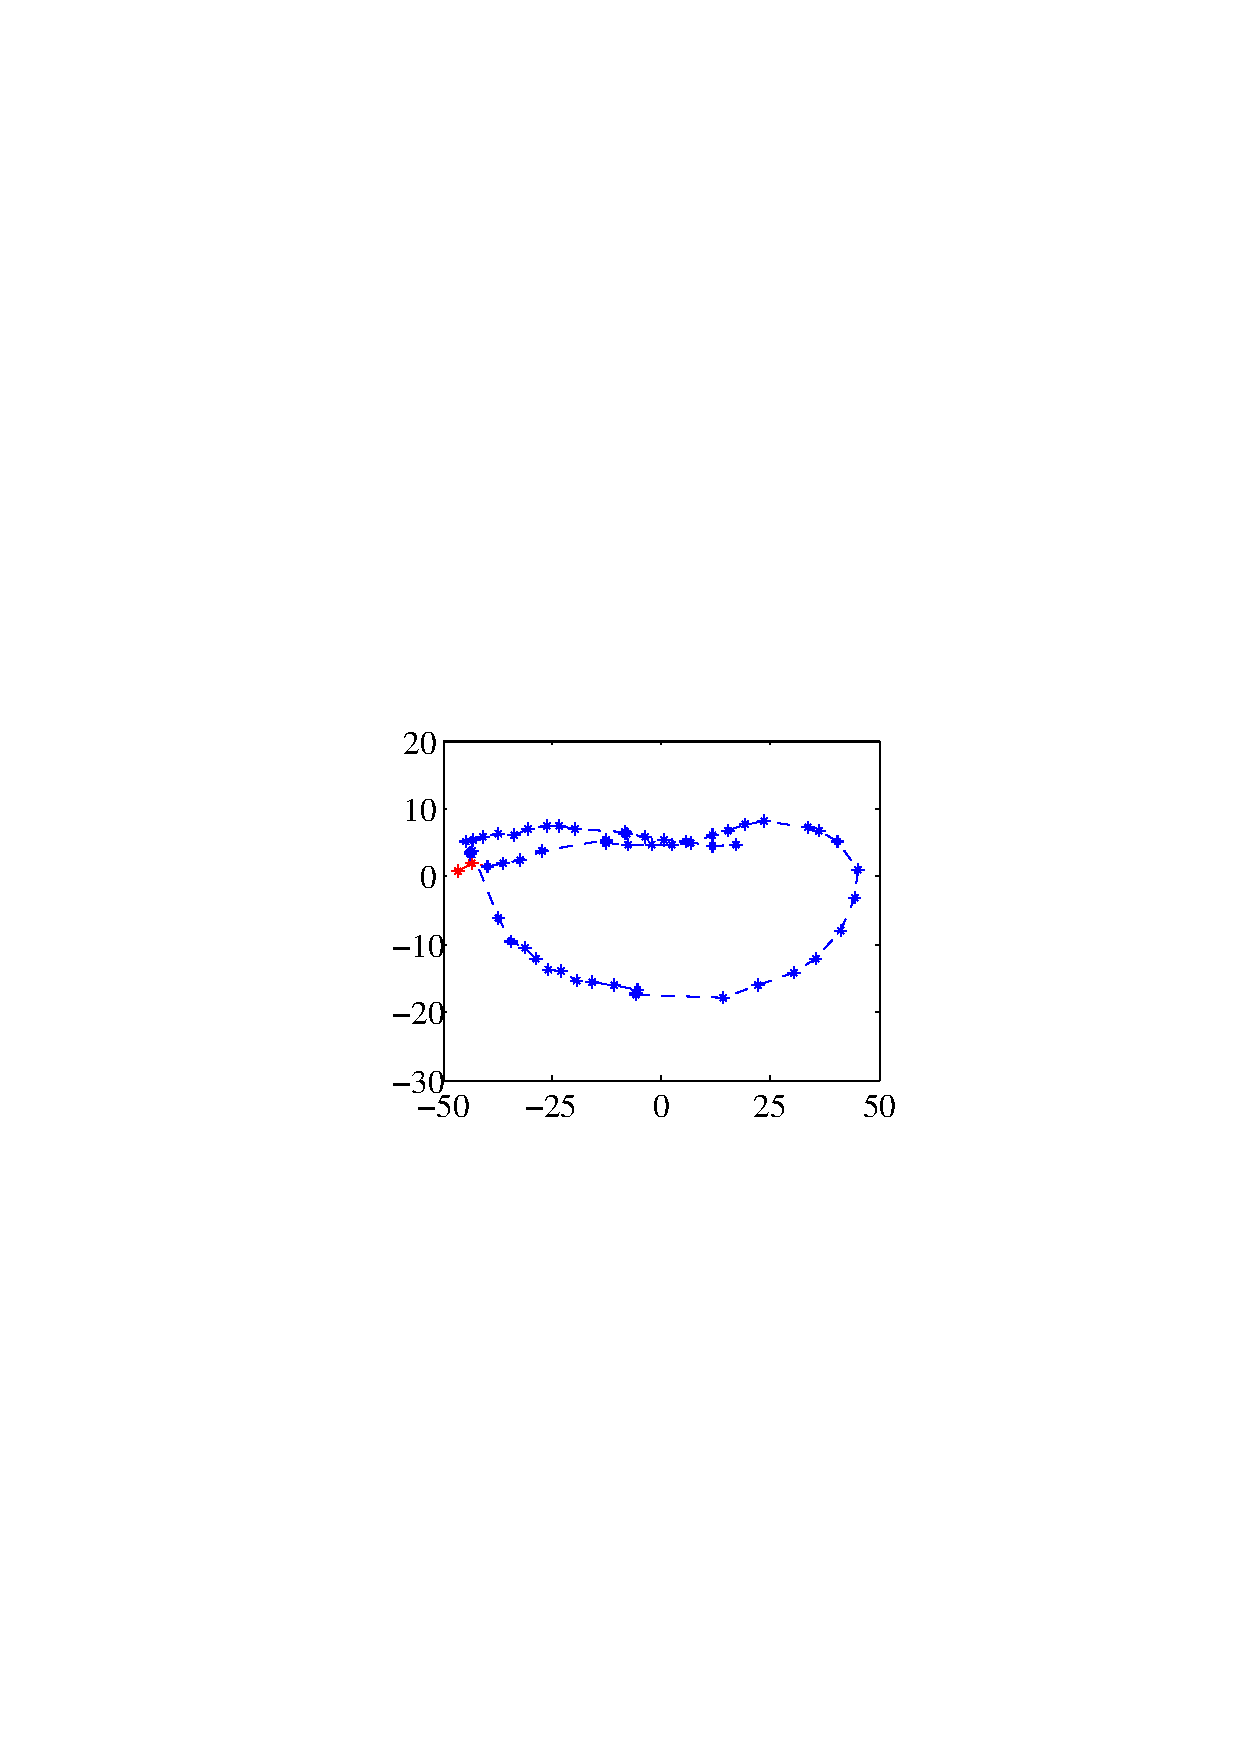
\includegraphics[width=\textwidth]{fig/gesture-distinction2.pdf}\\
            \centering  (b) two consecutively horizontal-swiping gestures
            \end{minipage}
        }
        %\vspace{-3mm}
        %\subfigure{
%            \begin{minipage}[t]{0.19\textwidth}
%            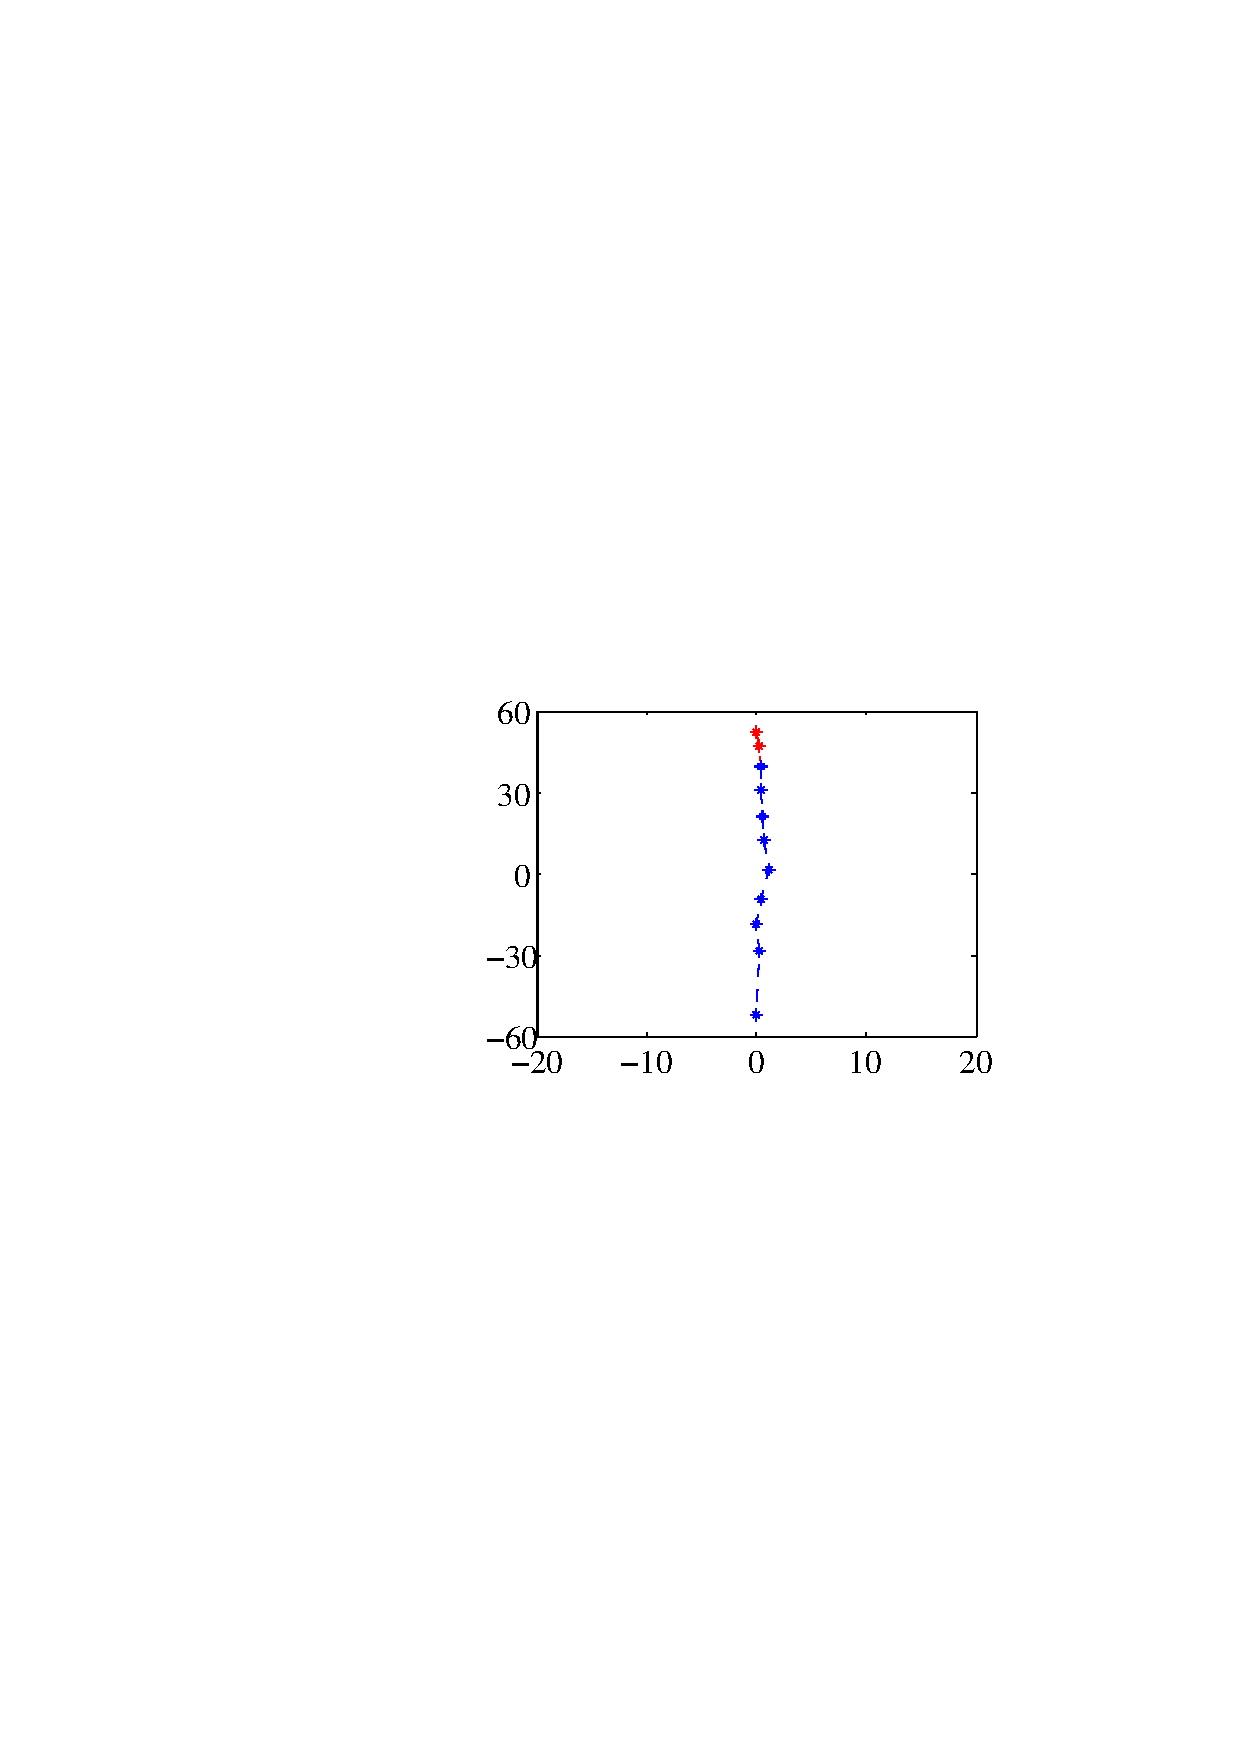
\includegraphics[width=\textwidth]{fig/gesture-distinction3.pdf}\\
%            \centering  (c) a vertical-swiping gesture
%            %\FIXME{Need to mark the starting point and turning point}
%            \end{minipage}
%        }
%        \hspace{0.25cm}
%        %\hfill
%        \subfigure{
%            \begin{minipage}[t]{0.19\textwidth}
%            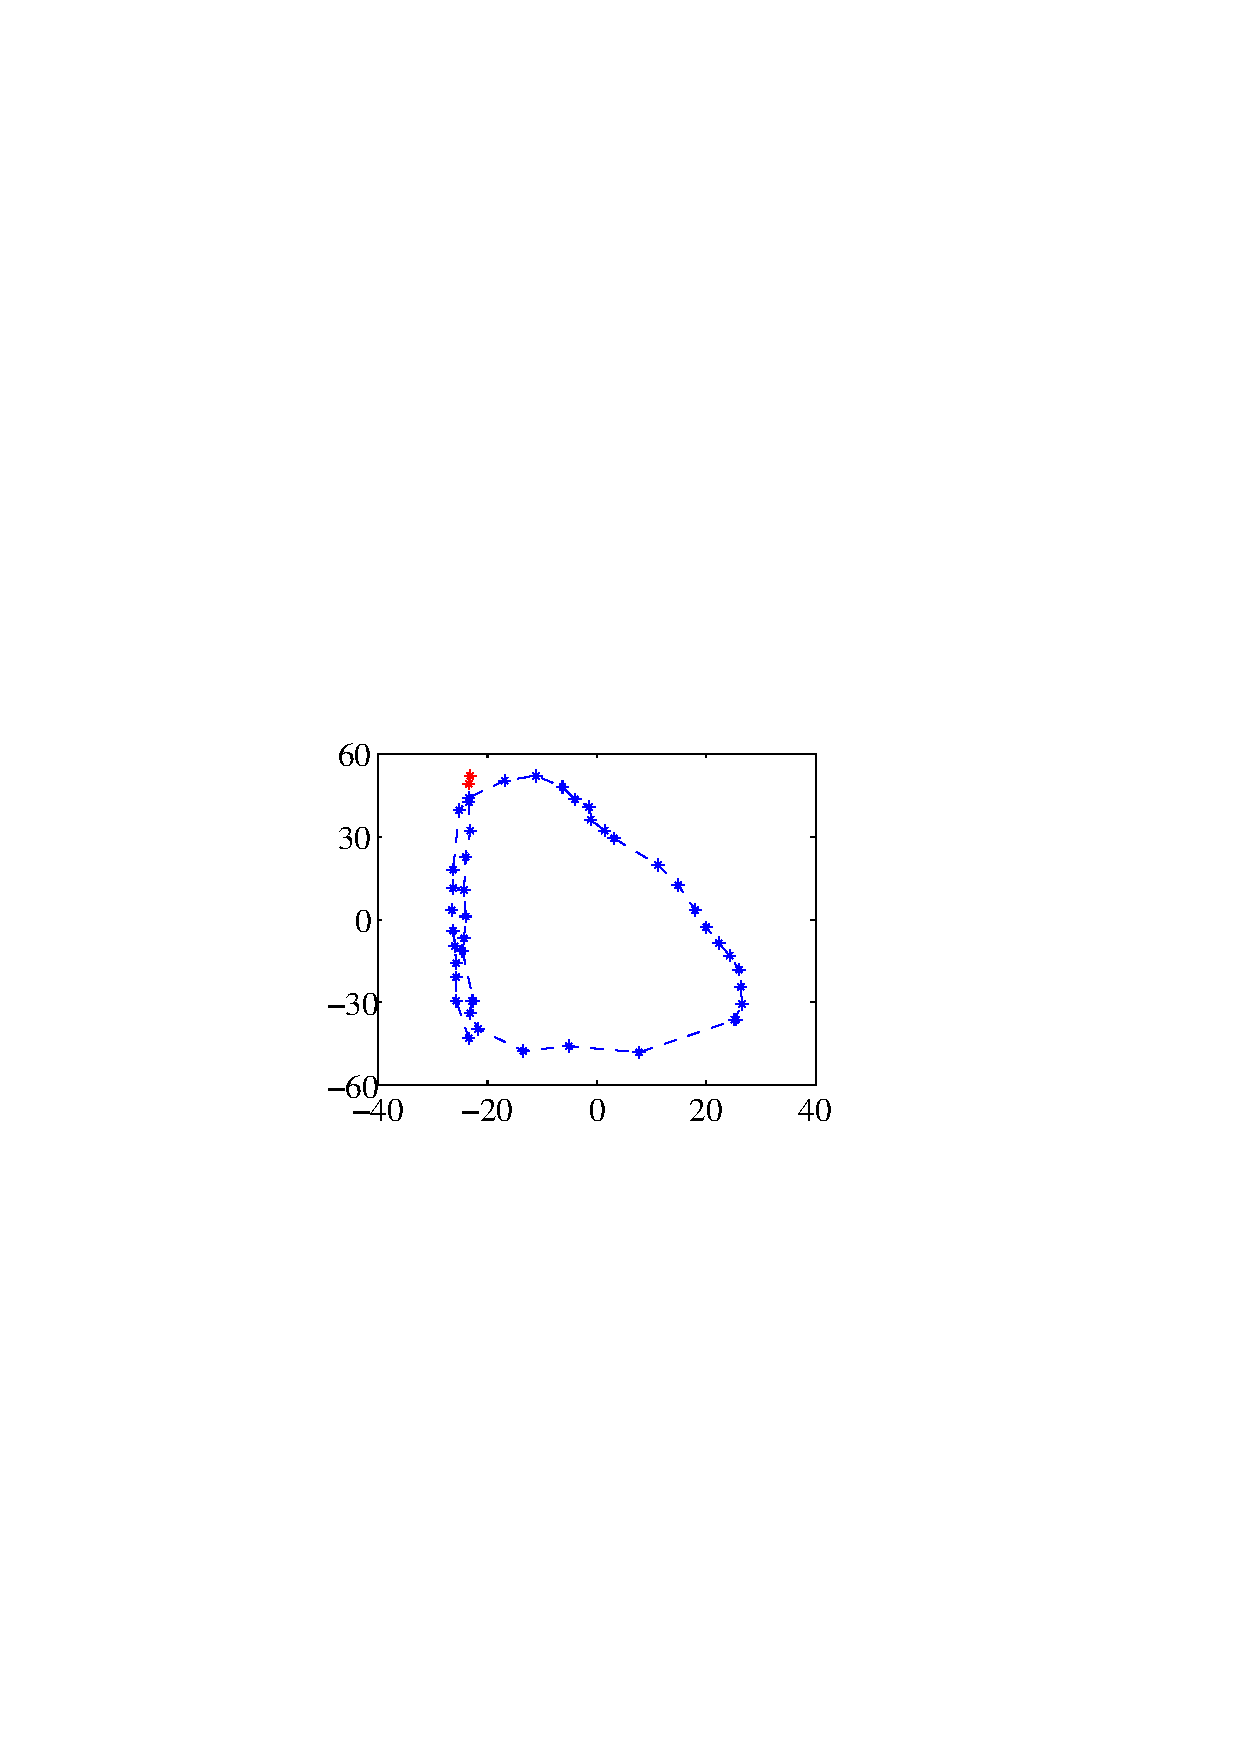
\includegraphics[width=\textwidth]{fig/gesture-distinction4.pdf}\\
%            \centering  (d) two consecutively vertical-swiping gestures
%            \end{minipage}
%        }
        \subfigure{
            \begin{minipage}[t]{0.19\textwidth}
            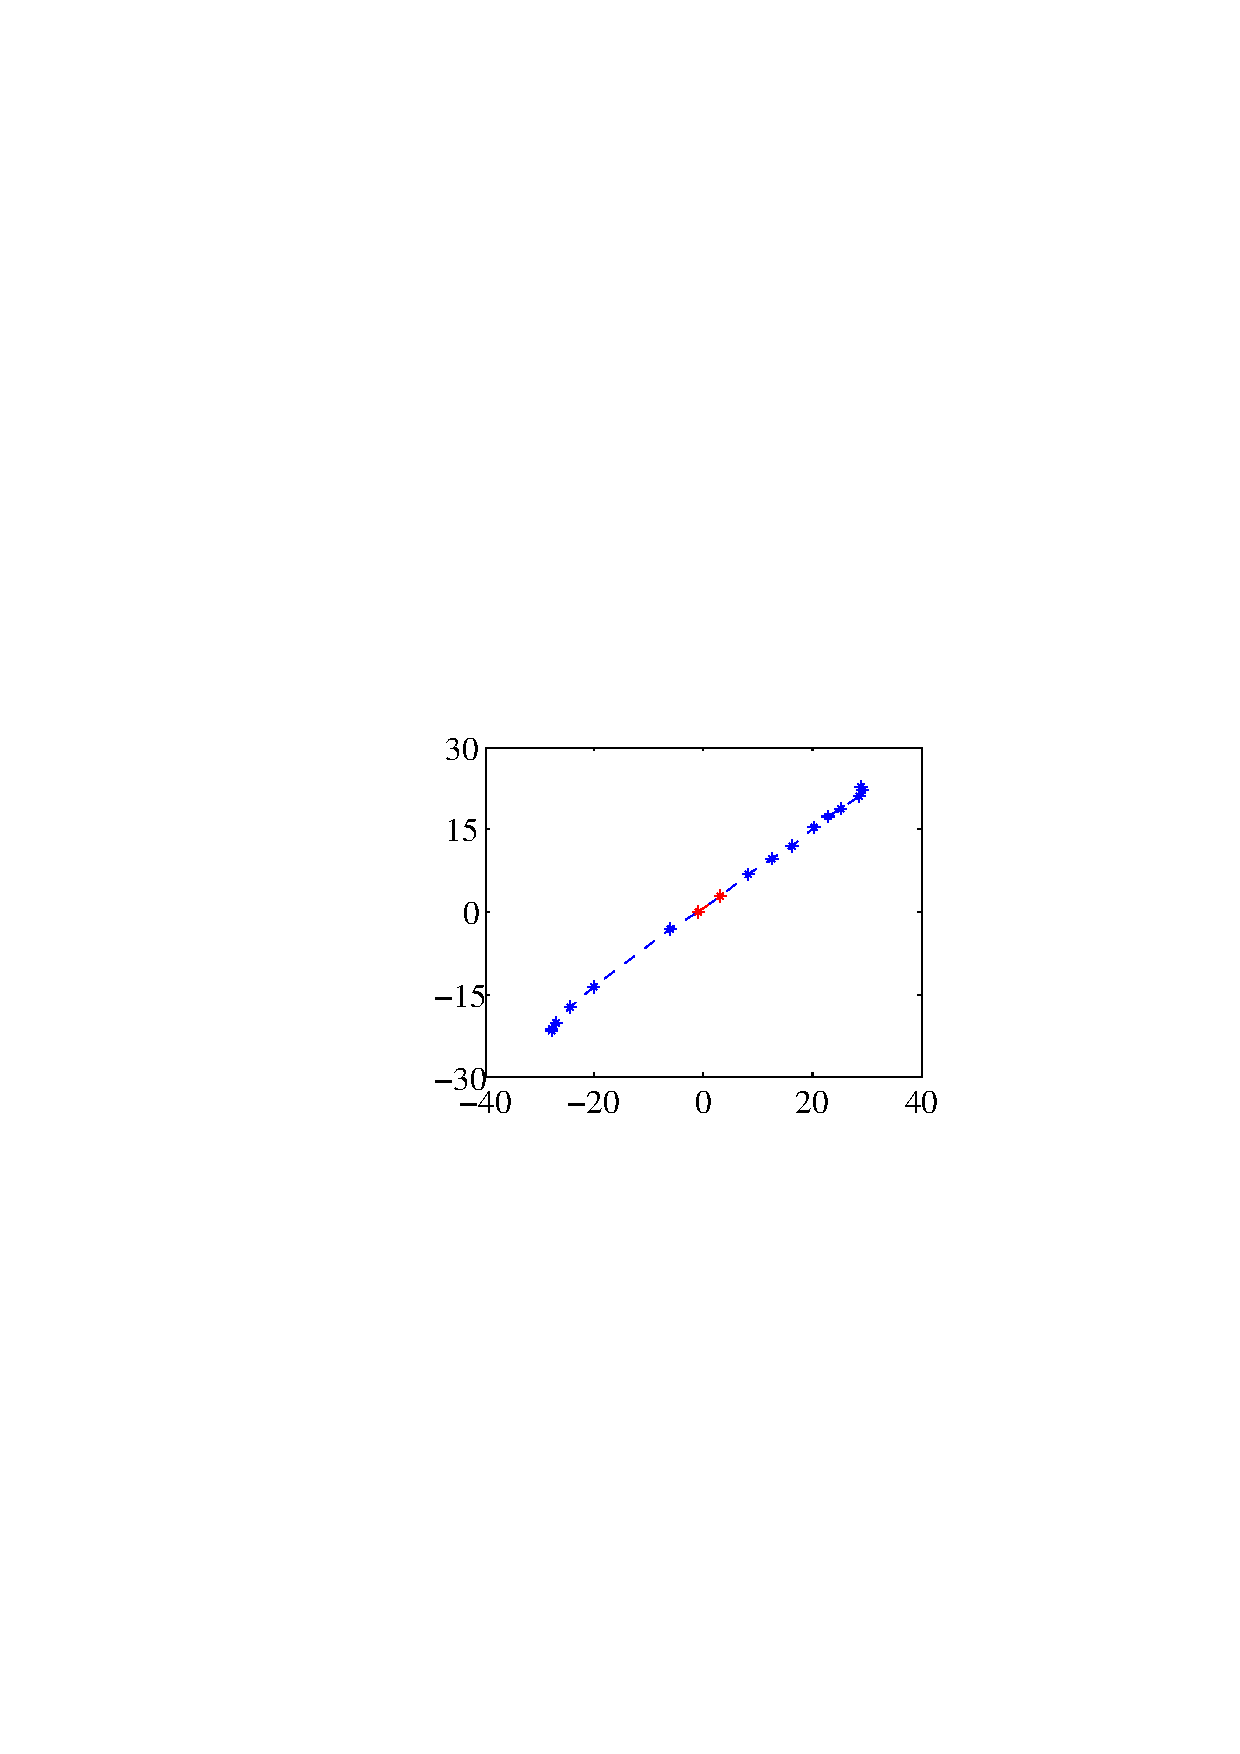
\includegraphics[width=\textwidth]{fig/gesture-distinction5.pdf}\\
            \centering  (c) a zooming gesture
            \end{minipage}
        }
        \vspace{-1mm}
        \hspace{0.25cm}
        %\hfill
        \subfigure{
            \begin{minipage}[t]{0.19\textwidth}
            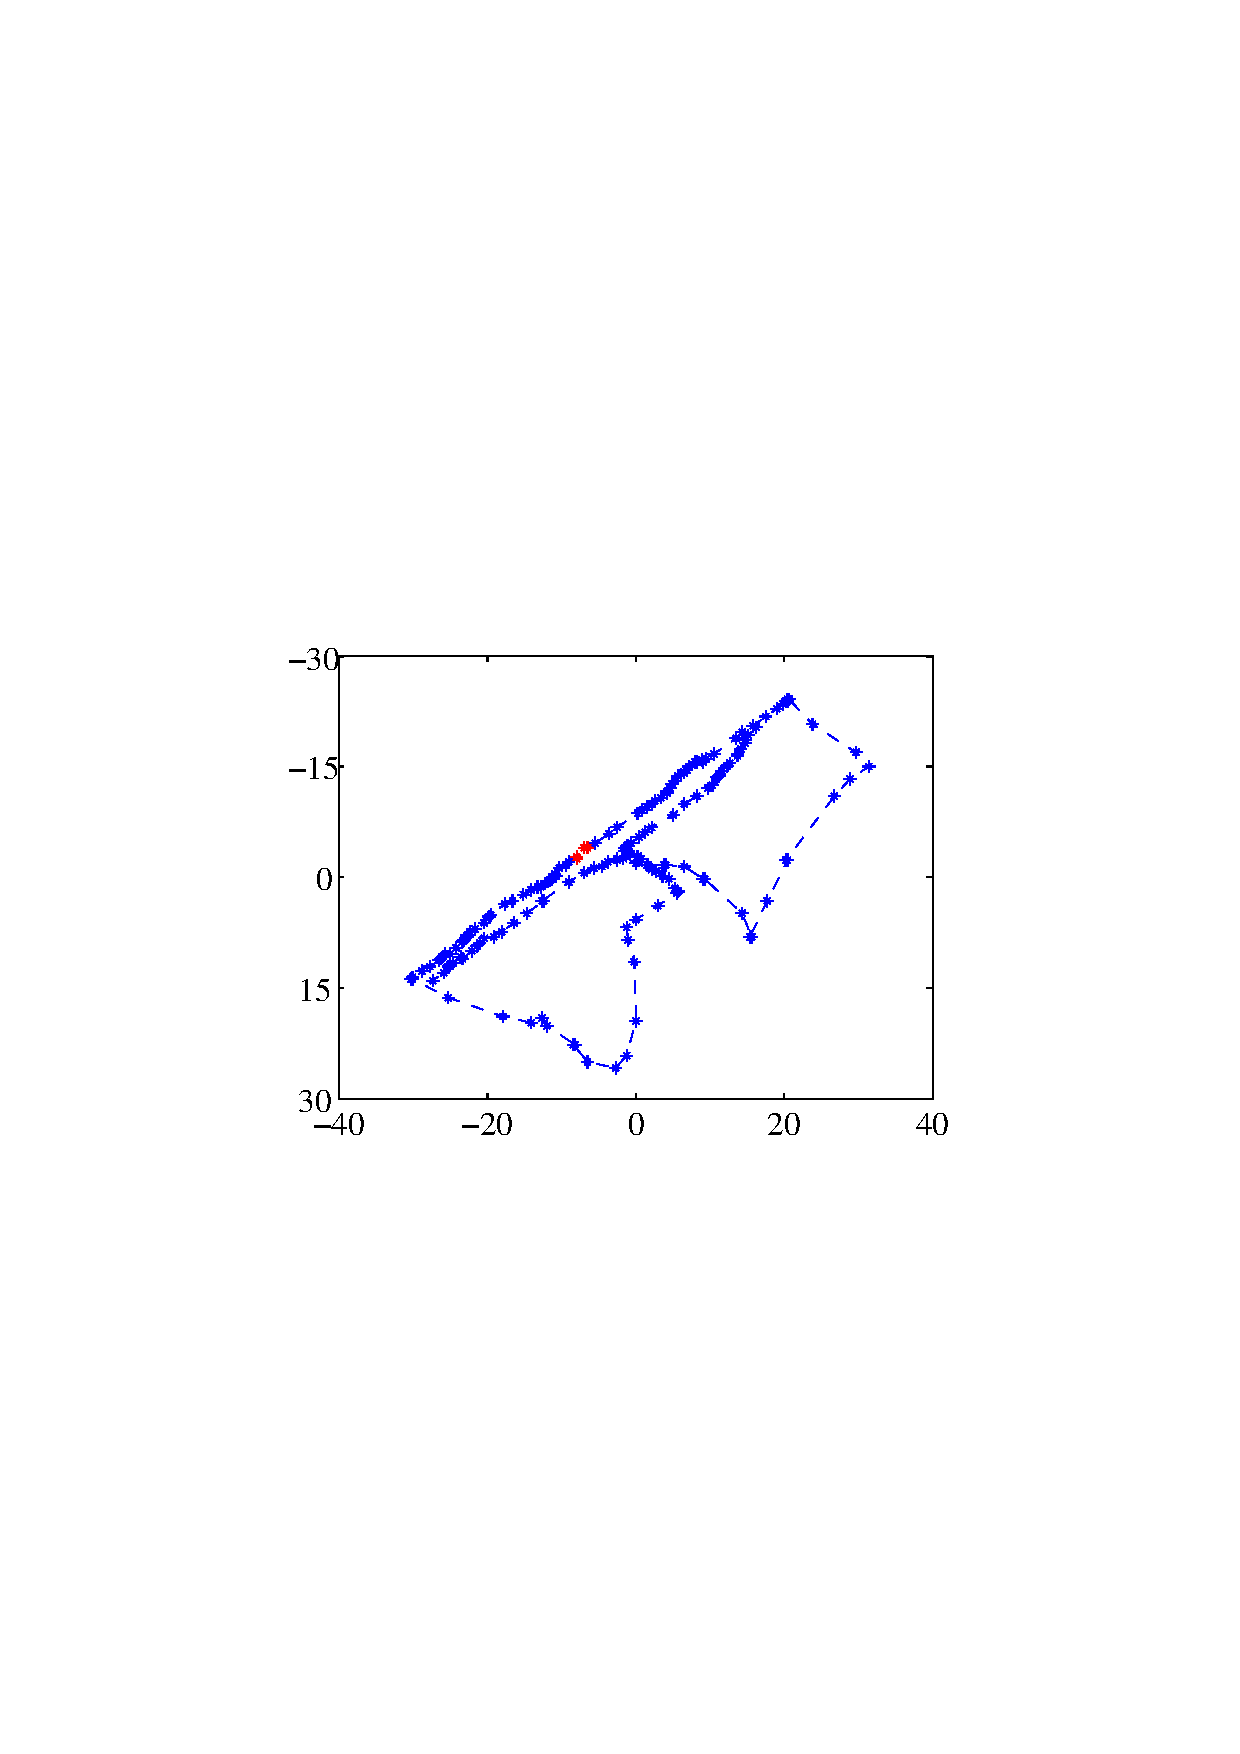
\includegraphics[width=\textwidth]{fig/gesture-distinction6.pdf}\\
            \centering  (d) two consecutive zooming gestures
            \end{minipage}
        }
        \vspace{-1mm}
        \caption{Spatial-temporal characteristics for performing an on-screen gesture once (a, c) and twice (b, d).}
        \label{fig:gesture-distinction}
        \vspace{-4mm}
    \end{figure}

        \begin{figure*}[!t]
            \centering
            \subfigure{
                \begin{minipage}[t]{0.23\textwidth}
                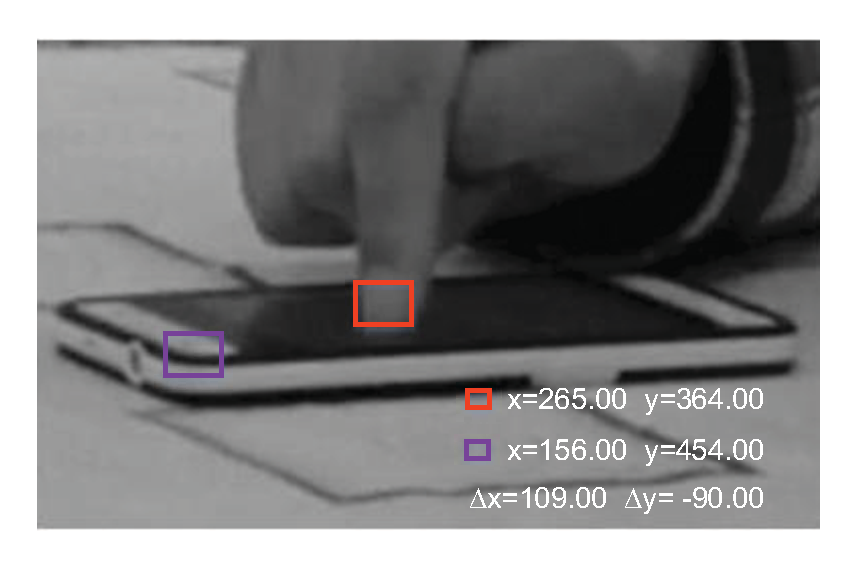
\includegraphics[width=1\textwidth]{fig/6--1.pdf}\\
                \centering  (a) The first video frame
                \end{minipage}
            }
            \hfill
            \subfigure{
                \begin{minipage}[t]{0.23\textwidth}
                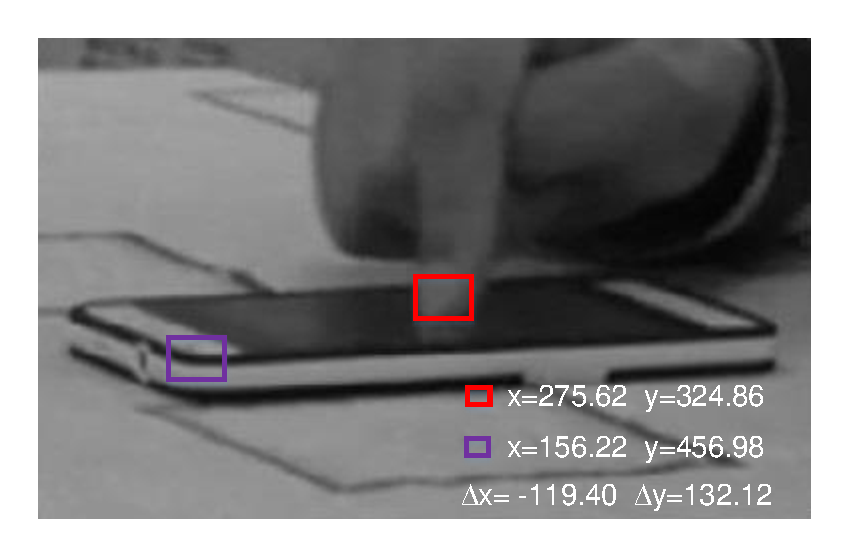
\includegraphics[width=1\textwidth]{fig/6--2.pdf}\\
                \centering  (b) A middle video frame
                \end{minipage}
            }
            \hfill
            \subfigure{
                \begin{minipage}[t]{0.23\textwidth}
                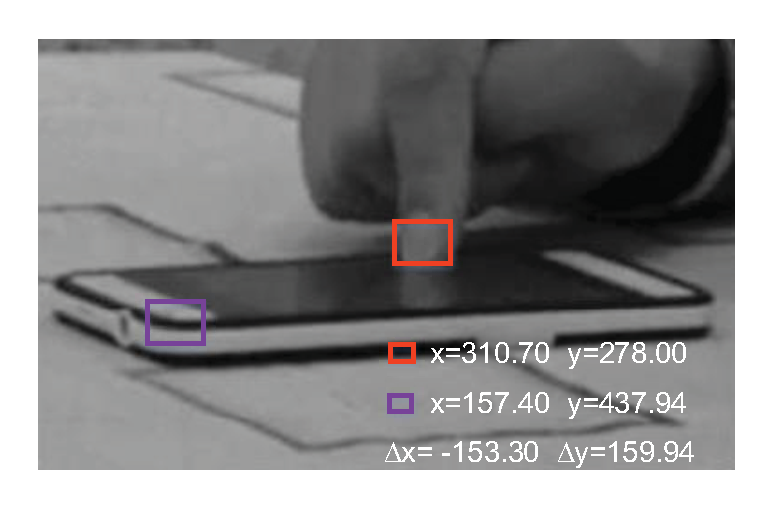
\includegraphics[width=1\textwidth]{fig/6--3.pdf}\\
                \centering  (c) The last video frame
                \end{minipage}
            }
            \hfill
            \subfigure{
                \begin{minipage}[t]{0.22\textwidth}
                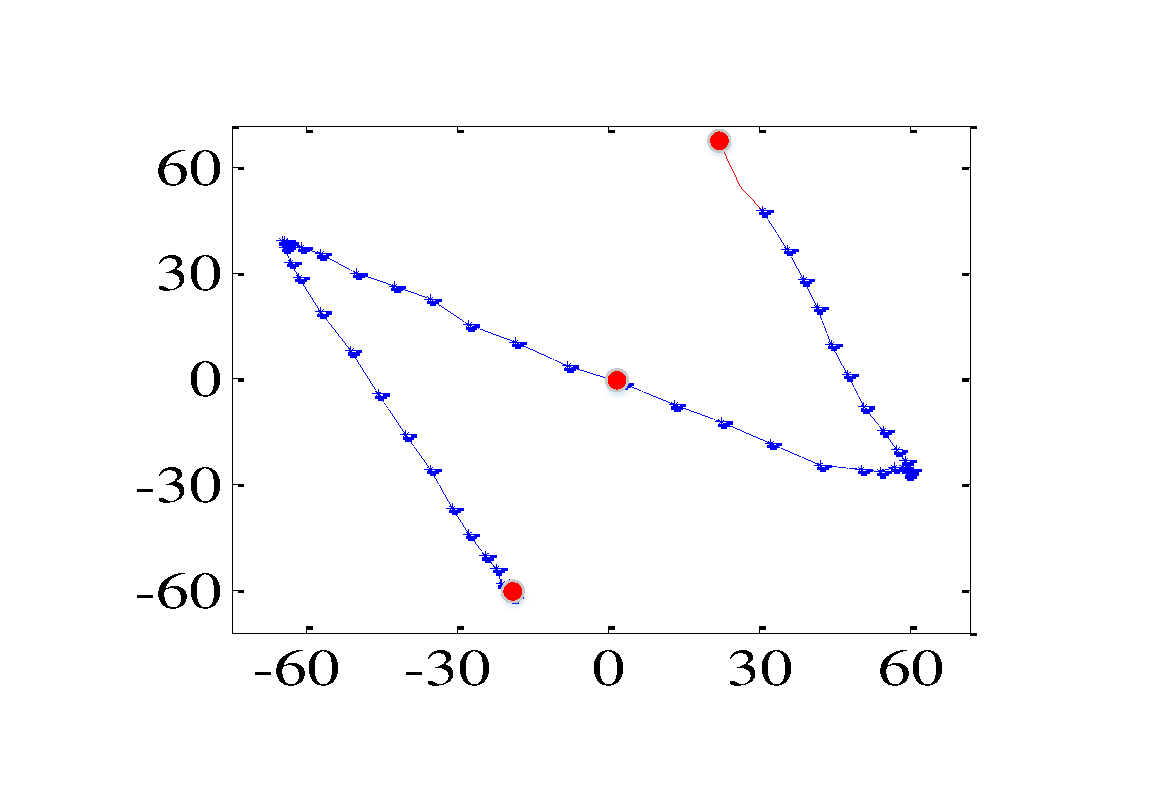
\includegraphics[width=1\textwidth]{fig/6--4.pdf}\\
                \centering  (d) Fingertip movement trajectory
                \end{minipage}
            }
            \vspace{-3mm}
            \caption{Tracking the fingertip movement trajectory. For each video frame, the system tracks two areas: one surrounds the fingertip and the other covers the edge of the device.
            The fingertip position is determined by computing the relative coordinates of the central points of the two areas.
            The red points highlighted in the final results (d) are the touching points tracked from the three video frames.}
            \label{fig:fig5}
            \vspace{-4mm}
        \end{figure*}

Our heuristic for identifying the pattern drawing process is described
in Algorithm~\ref{alg:recognition}. The input to the algorithm is a video capturing the unlocking process, and the output of the
algorithm is a time-stamp tuple, $<$start, end$>$, which marks the start and the end
of a video segment.
To locate the video segment of pattern drawing, we first filter out on-screen activities where the
fingertip location does not change within a timeframe of 1.5 seconds (lines 4 and 11). This
allows us to exclude some basic on-screen activities such as clicking. We
use the number of video frames, \emph{frameCount}, as a proxy to estimate the time interval between two on-screen operations. Here, a time
interval of 1.5s translates to 45 frames or 90 frames when the video was shot
at 30 or 60 frames per second (FPS) respectively. We also use the
spatial-temporal characteristics described above to exclude two consecutive swiping or zooming gestures (line 8). Finally, we exploit the observation that users
typically paused at least 1.5s before or after unlocking to locate the start
and end points of pattern drawing (line 19).

\noindent \textbf{Limitations} Our heuristic is not perfect. It is likely to fail if the user was typing
using a Swype-like method (i.e. entering words by sliding a finger from
the first letter of a word to its last letter) during video recording. In
this case, our method will identify multiple video segments of which one may contain
the pattern unlock process. If multiple segments are detected, the algorithm will ask the
user to confirm which video segment to use.
In this scenario, the first identified segment is likely to be the correct one.
In practice, an experienced attacker would wait patiently to avoid this
complicated situation by finding the right time for filming (e.g. for a screen
lock, the time is just after the device is retrieved).
The attacker could also watch the video to manually cut it to ensure to obtain the correct video segment.
%It is
%worthwhile to mention that automatically identifying the pattern unlocking process is
%not central to our attack because an attacker often can obtain a quality video input used the manual methods described above.
%Despite its limitations, our algorithm can reduce the efforts involved in some common scenarios.

    \begin{algorithm}[!t]
        \centering
        \caption{Unlocking process identification heuristic}
        %\FIXME{What is the threshold for fingertip location changes?}
        \label{alg:recognition}
        \begin{algorithmic}[1]
            \REQUIRE~~\\
                $IV$: Video footage  \\
                $frameCount$: Pause threshold before or after unlocking\\
                %$locationTh$: Threshold of fingertip location changes\\
            \ENSURE~~\\
                %$P[]$: Candidate patterns \\
                $<$start,end$>$: Start and end of the unlocking video segment \\
            \STATE $frames[] \leftarrow getVideoFrames(IV)$ \\
            \STATE $LEN \leftarrow getFramesLen(frames[])$ \\
            \FOR{$i=1:LEN-frameCount$}
                \STATE $sL \leftarrow hasFingertipChanged(frames[i:i+frameCount])$ \\
                \IF{$!sL$}
                    \STATE $sNo=i+frameCount$ \\
                    \FOR{$j=sNo:LEN$}
                        \IF{$checkLoop(frames[j:LEN])$}
                            \STATE $eNo=i$ \\
                            \STATE break; \\
                        \ELSIF{$!hasFingertipChanged(frames[j:j+frameCount])$}
                            \STATE $eNo=i$ \\
                            \STATE break; \\
                        \ENDIF
                    \ENDFOR
                    \STATE break;
                \ENDIF
            \ENDFOR
            \STATE $<start, end> \leftarrow getTargetVideo(frames[],sNo,eNo)$
        \end{algorithmic}
    \end{algorithm}

%    \begin{figure*}[!t]
%        \centering
%        \subfigure{
%            \begin{minipage}[b]{0.24\textwidth}
%            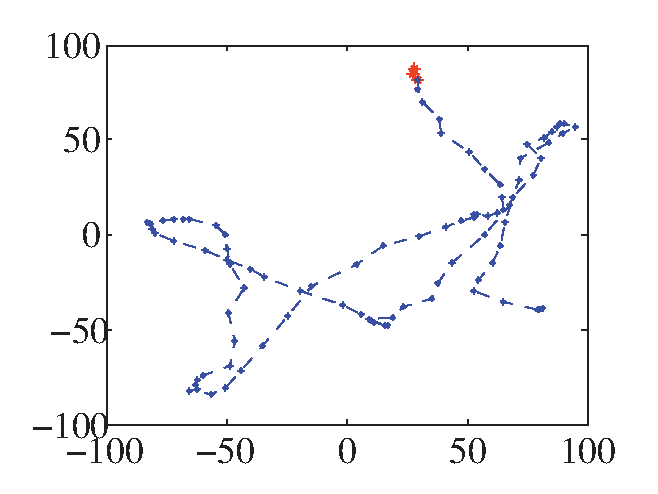
\includegraphics[width=\textwidth]{fig/5-1.eps}\\
%            \centering  (a) w/o camera shake calibration
%            \end{minipage}
%        }
%        \hfill
%        \subfigure{
%            \begin{minipage}[b]{0.24\textwidth}
%            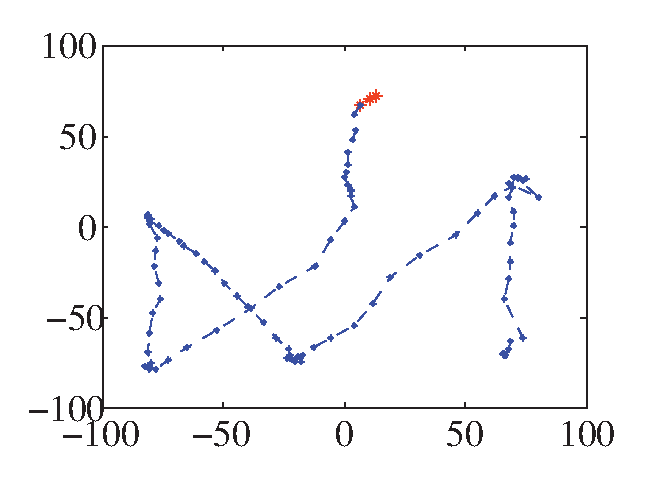
\includegraphics[width=\textwidth]{fig/5-2.eps}\\
%            \centering  (b) w/ camera shake calibration
%            \end{minipage}
%        }
%        \hfill
%        \subfigure{
%            \begin{minipage}[b]{0.18\textwidth}
%            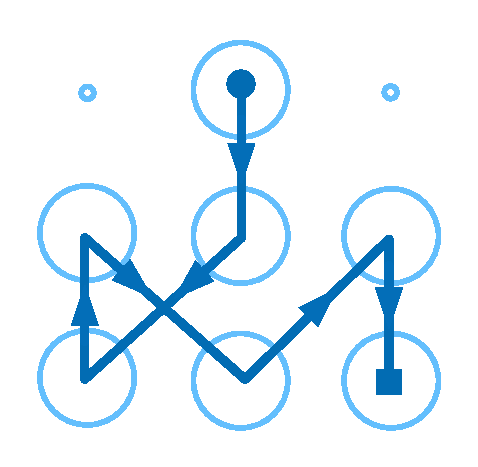
\includegraphics[width=\textwidth]{fig/5-3.pdf}\\
%            \centering  (c) correct pattern
%            \end{minipage}
%        }
%        \vspace{-3mm}
%        \caption{The resulted fingertip movement trajectories without (a) and with (b) camera-shake calibration.  The correct pattern is shown in (c). To aid clarity we have transformed (a) and (b) to the user's perspective.}
%        \label{fig:camera_shake_illu}
%        \vspace{-4mm}
%    \end{figure*}

\vspace{-3mm}
\subsection{Track fingertip locations}
\label{section:tld}

        After cutting out the video segment of pattern drawing, we need to track the finger motions from the video segment. We achieve this by employing a video tracking algorithm called
        \emph{Tracking-Learning-Detection (TLD)}~\cite{kalal2012tracking}. This
        algorithm automatically detects objects defined by a boundary box. In
        our case, the objects to be tracked are the user's fingertip and an area of the device.
        These are supplied to the algorithm by simply highlighting two areas on the first frame of the video segment (see Figure~\ref{fig:fig2} b). The
        algorithm tries to localize the fingertip from each video frame and aggregates the successfully tracked locations to produce a fingertip movement trajectory as an output (see Figure
        \ref{fig:fig2} c).

    \subsubsection{Generate The Fingertip Movement Trajectory}

        The TLD algorithm automatically detects
        objects based on the examples seen from the first frame.
        For each tracked object, the algorithm generates a confidence between 0 and 1.
        A tracking is considered to be successfully if the confidence is greater than a threshold.
        We set this threshold to 0.5 which is found to give good performance in our initial design experiments using 20 patterns\footnote{To provide a fair evaluation, the patterns used in
        our initial test runs in the design phase are different from the ones used later in evaluation.}.
        TLD has three modules: (1) a tracker that follows
        objects across consecutive frames under the assumption
        that the frame-to-frame motion is limited and objects are visible;
        (2) a detector to fully scan each individual frame to localize all
        appearances of the objects; and
        (3) a learner that estimates errors of the detector and updates the detector to avoid these errors in future
        frames.
%        The TLD learner automatically extracts features from the area of interest to build a K-Nearest Neighbor
%        classifier~\cite{hastie1996discriminant}
%        which is a part of the detector. In the following frames, the learner
%        estimates the detection errors and generates new training
%        examples (i.e. new appearances of the object) arose from object motion to
%        re-train the classifier to avoid these errors. For each video frame,
%        TLD calculates the tracking confidence and if the confidence is lower than the predefined threshold, the result of
%        this particular frame will be discarded. This allows the algorithm to
%        tolerate a certain degree of detection errors. Finally, the
%        successfully detected object locations will be put onto a single
%        image as the output.
        Detailed discussion of TLD can be found
        at~\cite{kalal2012tracking}.

         In some specific cases, the algorithm may fail to detect the objects in many video frames due to poor selections of interesting areas. If this happens, our system will ask the user to re-select the areas to track.
        We have also extended TLD to report when a
        fingertip position is seen on the footage. This temporal information is recorded as the number
        of video frames seen with respect to the first frame of the video segment.
        This is used to separate two possibly overlapping line segments described in Section~\ref{section:spea}.



\begin{figure}[!t]
    \centering
    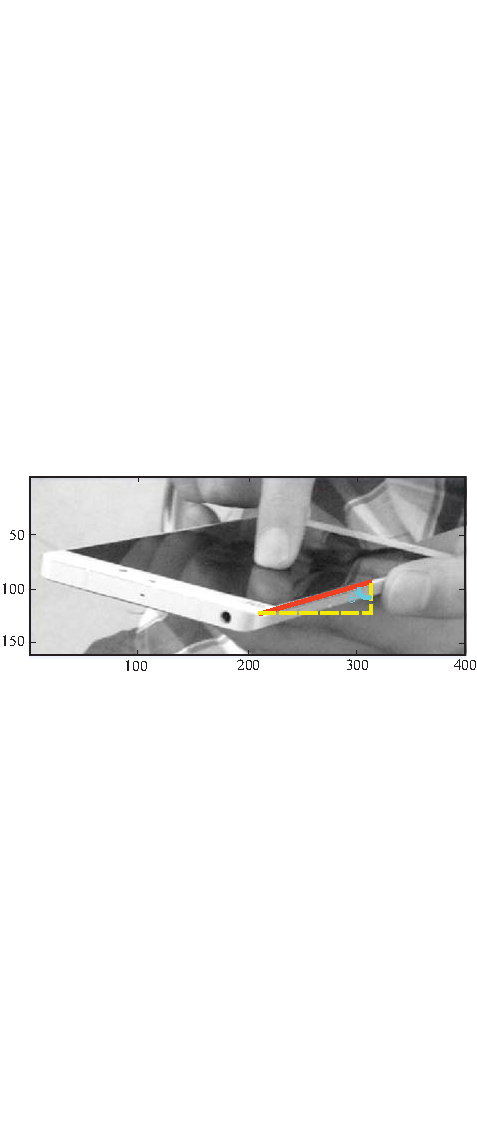
\includegraphics[width=0.45\textwidth]{fig/line_detection.pdf}
    \caption{Filming angle calculation. The filming angle, $\theta$, is the angle between the edge line of the device and a vertical line.}
    \label{fig:line_detection}
    \vspace{-5mm}
\end{figure}

        \subsubsection{Camera Shake Calibration}
        \label{secction:shake}
         By default, the TLD algorithm reports the position of a tracked object with respect to the top-left pixel of the video frame.
         However, videos recorded by a hand-held device are not always perfectly steady due to
        camera shake. As a result, the top-left pixel of a video frame may appear in a different location in later frames.
        This can drastically affect the precision of fingertip localization, leading to misidentification of patterns.

        Our approach to cancel camera shake is to record the fingertip
        location with respect to a fixed point of the target device. To do so, we track two
        areas from each video frame. One area is an edge of the device and
        the other is the fingertip. Both areas are highlighted on the
        first frame by the user.
        The location of a successfully tracked fingertip is reported as
        the relative coordinates of the two center points of the marked areas.
        This approach can also be used to calibrate the minor motions of the target device during pattern drawing.

        \noindent \emph{Example:} To illustrate how our camera-shake calibration method  works, considering
        Figure~\ref{fig:fig5} where two areas are firstly marked by two
        bounding boxes in subfigure (a).
        Both areas will
        then be automatically detected by the TLD algorithm in following video
        frames as shown in subfigures (b) and (c).
        The coordinates of the two center points of each box are the values of $x$ and $y$, and their relative positions are represented by
        $\triangle X$ and $\triangle Y$.
        For each frame
        where both areas are successfully tracked, we
        compute the relative coordinates, ($\triangle X$, $\triangle Y$), which are reported as the location of the tracked fingertip.

%        Figure~\ref{fig:camera_shake_illu} shows the results when using TLD to process a video that was filmed with some camera shake effects.
%        Figure~\ref{fig:camera_shake_illu} illustrates the tracking results without (a) and with (b) camera-shake calibration.
%        To aid clarity, we have
%        converted the trajectories into the user's perspective. Without
%        camera-shake calibration, the resulted trajectory is significantly different from the actual pattern shown in Figure~\ref{fig:camera_shake_illu} (c).
%        Because of this great difference, using Figure~\ref{fig:camera_shake_illu} (a)  will lead to misidentification of
%        candidate patterns. By contrast, Figure~\ref{fig:camera_shake_illu} (b) generated with camera-shake calibration is more alike the correct pattern.

      %  \subsubsection{Noisy Points Calibration}
%            During tracking process, the TLD algorithm may report mistaken position of a tracked object as rapid deformation of the tracked object. This can affect the shape of fingertip movement, leading to extract incorrect geometric information of fingertip movement.

\vspace{-3mm}
\subsection{Filming angle transformation}
\label{sec:transformation}
In practice, the filming camera will not directly face the target device to avoid raising suspicion by the target user. As a result, the
fingertip movement trajectory generated by the tracking
algorithm will look differently from the actual pattern. For example, for the
pattern presented in Figure~\ref{fig:fig2} (a), if the video is filmed from the attacker's front-left to the target device (i.e. with a filming angle of approximate 45 degrees),
we get the trajectory shown in Figure~\ref{fig:fig2} (c).
Using this trajectory without any postprocessing will lead to misidentification of candidate patterns.
Therefore, we must transform the resulting trajectory to the user's view point. To do so, we need to estimate the angle between the filming camera and the target device. Our approach is described as follows.

We use an edge detection algorithm called Line Segment Detector (LSD)~\cite{grompone2010lsd} to detect the longer edge of the device.
The filming angle is the angle between the detected edge line and a vertical line. This is illustrated in Figure~\ref{fig:line_detection}.
%In Section~\ref{sec:angle}, we show that a minor estimation error of the filming angle has little impact on the attacking success rate.
%By default, we assume that the pattern grid is presented in the portrait
%mode\footnote{The pattern grid of the Android native pattern lock is always presented in the portrait mode regardless of the orientation of the device.}. If this is
%not the case, i.e. the pattern grid is shown in the landscape mode, we need
%to use the shorter edge of the device to calculate the filming angle. We believe that an attacker interested in a particular target device would
%have some knowledge of how the pattern grid is presented under different orientation modes and be able to identify the device orientation by watching the video.
There are also other methods to be used to identify the filming angle~\cite{Torralba:2002:DEI:628330.628820}.

%\renewcommand{\algorithmicforall}{\textbf{for each}}
%    \begin{algorithm}[!t]
%        \caption{Candidate Pattern Identification Algorithm}
%        \label{alg:alg1}
%        \begin{algorithmic}[1]
%            \REQUIRE~~\\
%                $L[]$: Relative line length \\
%                $D[]$: Direction number (see Figure~\ref{fig:fig7}) \\
%                $tn$: Number of turning points of fingertip trajectory \\
%                %$timeTh$ Threshold of considering the turning points.\\
%                $lengthTh$: Threshold of considering two lines to have the same length\\
%                $directionTh$: Threshold of considering two lines to be in the same direction\\
%            \ENSURE~~\\
%                $P[]$: Candidate patterns \\
%
%            \FOR{\textbf{each} possible pattern $p$ with $tn$ turning points}
%                \STATE $n \leftarrow getLineNumber(P[])$ \\
%                \STATE $pL[]  \leftarrow getRelativeLength(p)$ \\
%                /*Relatvie line length for pattern $p$*/ \\
%                \STATE $pD[] \leftarrow getDirection(p)$ \\
%                \IF{match($pL[]$, $L[]$, $lengthTh$)}
%                    \IF{match($pD[]$, $D[]$, $directionTh$)}
%                        \STATE $P[] \leftarrow p$\\
%                    \ENDIF
%                \ENDIF
%            \ENDFOR
%            \STATE $P[] \leftarrow sort(P[])$
%        \end{algorithmic}
%    \end{algorithm}

Based on the estimated filming angle, $\theta$, we use the following formula to transform the tracked fingertip movement trajectory from the camera's view point to the user's:

\begin{equation}
        S=TS^{'} \qquad, \qquad  T=\left[ \begin{matrix} \cos\theta & -\sin\theta \\ \sin\theta & \cos\theta \end{matrix} \right]
\end{equation}

where $T$ is a Transformation Matrix, $S^{'}$ is the coordinate of a point of the tracked trajectory, and $S$ is the resulting coordinate after the transformation.
For each video frame, our algorithm individually calculates the filming angle and perform the transformation, because the filming angle may change across video frames.

%\renewcommand{\algorithmicforall}{\textbf{for each}}
%    \begin{algorithm}[!t]
%        \caption{Line Segment Identification}
%        \label{alg:turning-point}
%        \begin{algorithmic}[1]
%            \REQUIRE~~\\
%                \textbf{struct} $T[]$: Temporal information of each tracked location\\
%                $timeTh$: Threshold of whether two line segments are overlapping \\
%            \ENSURE~~\\
%                $tp[]$ Turning points of fingertip movement. \\
%            \FOR{\textbf{each} fingertip movement with temporal sequences $T[]$}
%                \STATE $tpNum=0$; \\
%                \STATE \textbf{struct} $lines[] \leftarrow getLines(T[]) $ \\
%           % \FOR{\textbf{each} t in $T[]$}
%                \STATE $lNum \leftarrow getLinesNumber(lines[])$ \\
%                \FOR{$i=1:lNum$}
%                    %\STATE $tp[tpNum] \leftarrow getStartingPoints(lines[i],timeTh)$ \\
%                    \IF{$checkOverlap(lines[i],timeTh)$}
%                        \STATE $p[tpNum++] \leftarrow getOverlapPoints(line[i])$ \\
%                    \ENDIF
%                    \STATE $p[tpNum++] \leftarrow getTurningPoints(line[i])$ \\
%                \ENDFOR
%            \ENDFOR
%            \STATE $tp[]=p[0:end-1]$\\
%        \end{algorithmic}
%    \end{algorithm}

\vspace{-3mm}
\subsection{Identify and rank candidate patterns}
\label{section:spea}
  In this step, the fingertip movement trajectory will be mapped to a number of candidate patterns to be tested on the target device.
   Our goal in this step is to exclude as many patterns as possible and only leave the most-likely patterns to be tried out on the target device.
     Our approach is to use the geometry information of the fingertip movement trajectory, i.e. the length and direction of line segments and the number of turning points, to reject patterns that do not satisfy certain criteria.
    In this section, we first describe how to identify overlapping line segments and extract length and direction information before presenting how to use the extracted information to identify and rank candidate patterns.

    \begin{figure}[!t]
        \centering
        \subfigure{
            \begin{minipage}[b]{0.23\textwidth}
            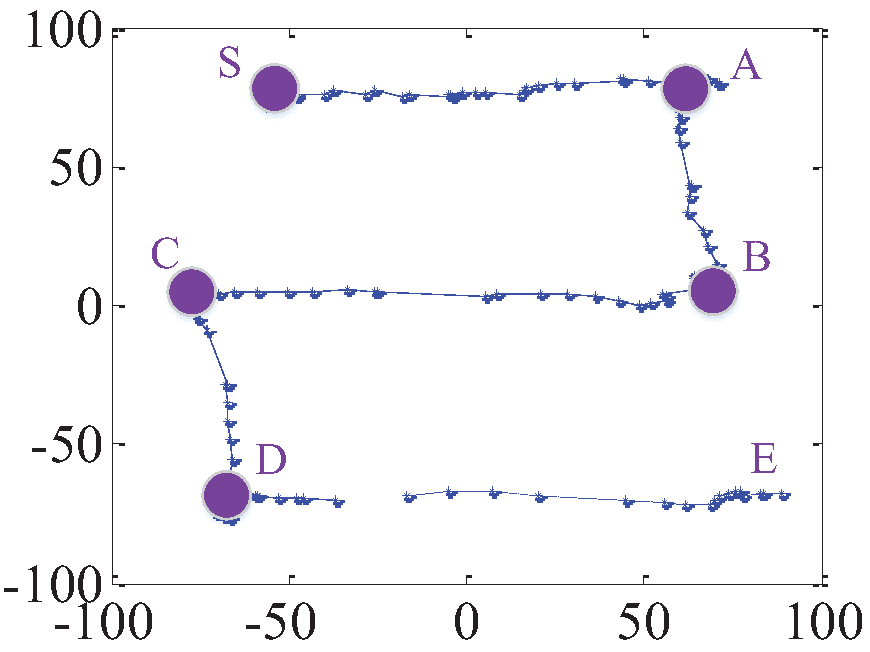
\includegraphics[width=\textwidth]{fig/6-2.pdf}\\
            \centering  (a) tracked fingertips
            \end{minipage}
        }
        \hspace{0.2cm}
        \subfigure{
            \begin{minipage}[b]{0.18\textwidth}
            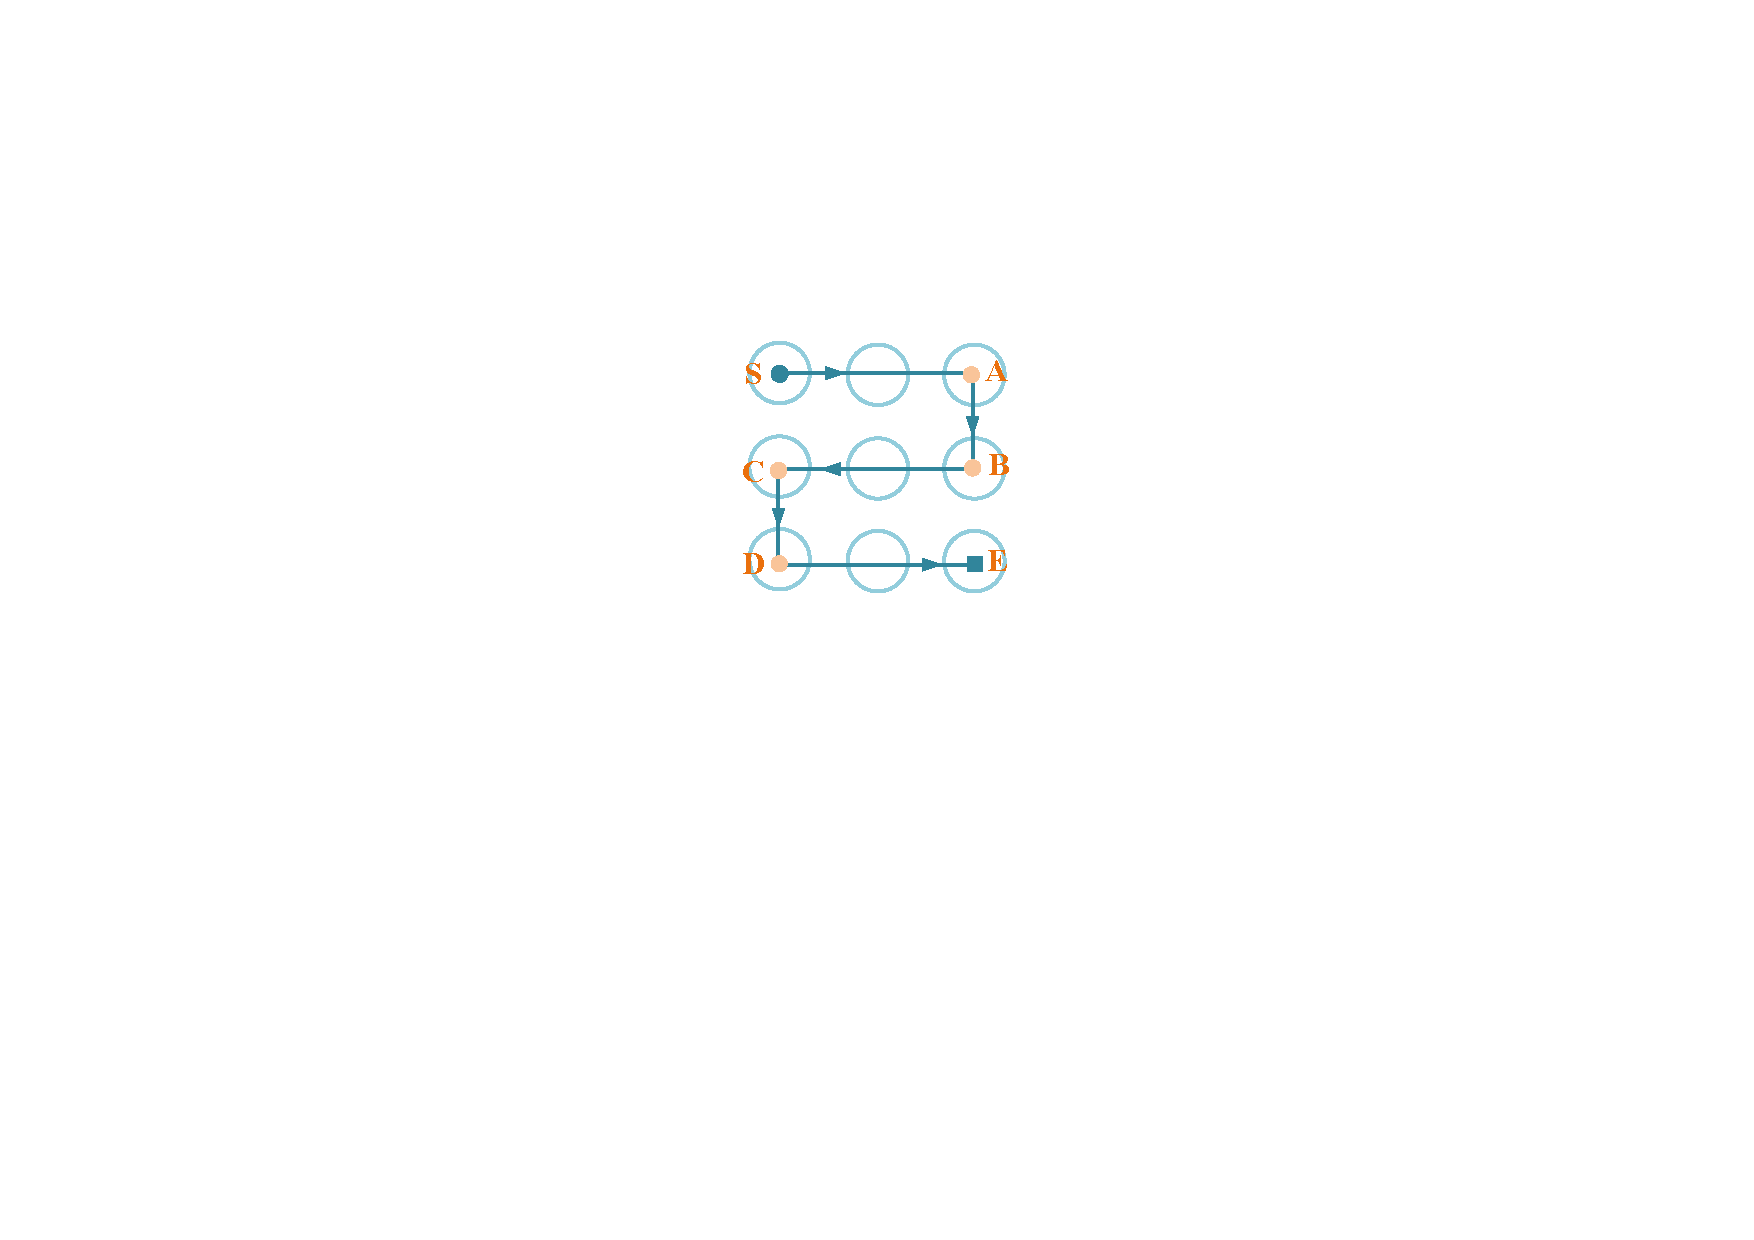
\includegraphics[width=\textwidth]{fig/6-1.pdf}\\
            \centering  (b) pattern example
            \end{minipage}
        }
        \caption{This figure shows the tracked fingertip movement trajectory (a) of a pattern (b). Point S on (a) is the starting point and points A, B, C, and D on (b) represent four turning points.}
        \label{fig:fig6}
        \vspace{-4mm}
    \end{figure}

    \subsubsection{Extracting Structure Information}
        A pattern can be defined as a collection of line
        segments where each line segment has two properties:
        the length of the line, $l$, and the direction of the line, $d$.
        We define a
         pattern, $P$, as a collection of line segment prosperities,  $P=\{L, D\}$.
        Here $L=\{l_{1}, l_{2}, \cdots, l_{n}\}$ is a collection of the lengths
        of all line segments (that are numbered from $1$ to $n$) of the pattern, and $D=\{d_{1}, d_{2}, \cdots, d_{n}\}$ is the collection of directions for all line segments in $L$.
        %Algorithm~\ref{alg:alg1} describes how $P$ is extracted.
        We extract the length and the direction of each line segment from the tracked fingertip movement trajectory and store them
        into arrays $L[]$ and $D[]$ respectively.

        \noindent \textbf{Identify Line Segments.}
        The first step of geometry information extraction is to identify individual
        line segments from the trajectory. This can be achieved
        by finding turning points, the start and the end points of the pattern, because two points define a line segment. For example, turning points, A and B, in
        Figure~\ref{fig:fig6} defines a line segment, AB.
        %In Algorithm~\ref{alg:turning-point},
        We use a linear fitting
        method~\cite{Kutner2004Applied} to discover turning points. %(line 3).
        A specific challenge here is how to separate two overlapping line segments
        %(see Figure~\ref{fig:intersection-overlap} c for an example).
        It is to note that up to two lines can be overlapped on a pattern grid.
        The naive
        linear fitting algorithm would consider two overlapping segments to be a
        single line as their points stay close to each other. We overcome this problem
       by using the temporal information (that is recorded by the
        tracking algorithm) to separate two overlapping points.
%        To do so, we visit all tracked points of each line segment given by the linear fitting algorithm (line
%        5) within a timeframe (\emph{timeTh}) of 20 video frames for a video of 30 FPS (40 for a video of 60 FPS).
%        For each point, we calculate its Euclidean distances to all other points within the timeframe.
%        We consider two points to be overlapping if their distance is less than 5 pixels.
%        For a video shot at 30 FPS, we consider there exist two overlapping line segments if 5 (10 for a 60 FPS video) or more overlapping points in the timeframe.
%        Again, these threshold values were determined through our initial design experiments.
%        Finally, we consider the center of all points as the turning point of the two overlapping line segments and use turning point to separate the two lines.

        \noindent \emph{Example:} As an example, consider a fingertip movement trajectory shown in
        Figure~\ref{fig:line-idenfication} (a). The red rectangle on the
        figure is a timeframe consisting of 20 tracked points.  If we zoom in
        on the timeframe, we get Figure~\ref{fig:line-idenfication} (b) where
        a point is labelled with a frame number according to when
        the point was seen, starting from 1 for the earliest point. In this example, there are more than 6
        overlapping points in the timeframe, which are marked by a green
        circle. We use the center
        point (No.10) of the overlapping points as the turning point to separate the two line segments.

        \begin{figure}[!t]
            \centering
            \subfigure{
                \begin{minipage}[b]{0.23\textwidth}
                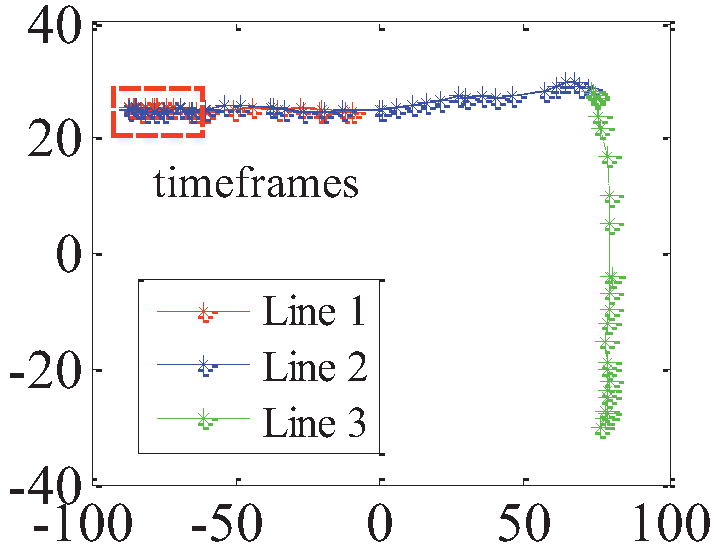
\includegraphics[width=\textwidth]{fig/line-identification1.pdf}\\
                \centering  (a) overlapping lines
                %\FIXME{Need to mark the starting point and turning point}
                \end{minipage}
            }
            \subfigure{
                \begin{minipage}[b]{0.225\textwidth}
                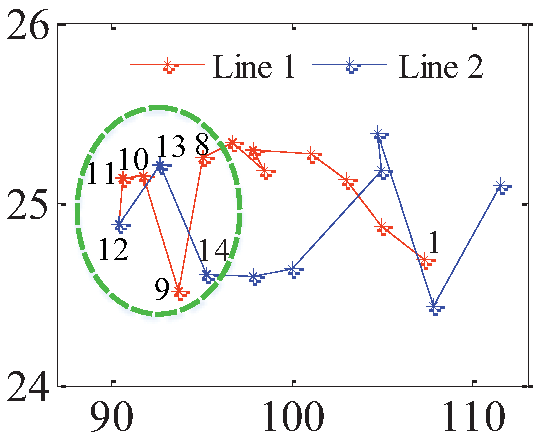
\includegraphics[width=\textwidth]{fig/line-identification2.pdf}\\
                \centering  (b) zoom-in view
                \end{minipage}
            }
            \caption{Separating two overlapping line segments by checking the number of overlapping points within a timeframe.}
            \label{fig:line-idenfication}
            \vspace{-3mm}
        \end{figure}
        \noindent \textbf{Extract the Line Length.}
        The physical length of a line segment depends
        on the sizes of the screen and the pattern grid, and the space between two touch dots.
        To ensure our approach is independent of the device, we normalize the physical length of a line segment to the
        shortest line found on the tracked trajectory. For the
        example shown in Figure~\ref{fig:fig6} (a), the line lengths for segments, SA, AB, BC, CD, and DE, are $2l_{s},l_{s},2l_{s},l,2l_{s}$, respectively.
        Here segments AB and CD have the shortest length, $l_s$. The physical length of a line segment is calculated by computing the
        Euclidean distance between the start and the end points of a segment.

        \begin{figure}[!t]
            \centering
            \subfigure{
                \begin{minipage}[t]{0.2\textwidth}
                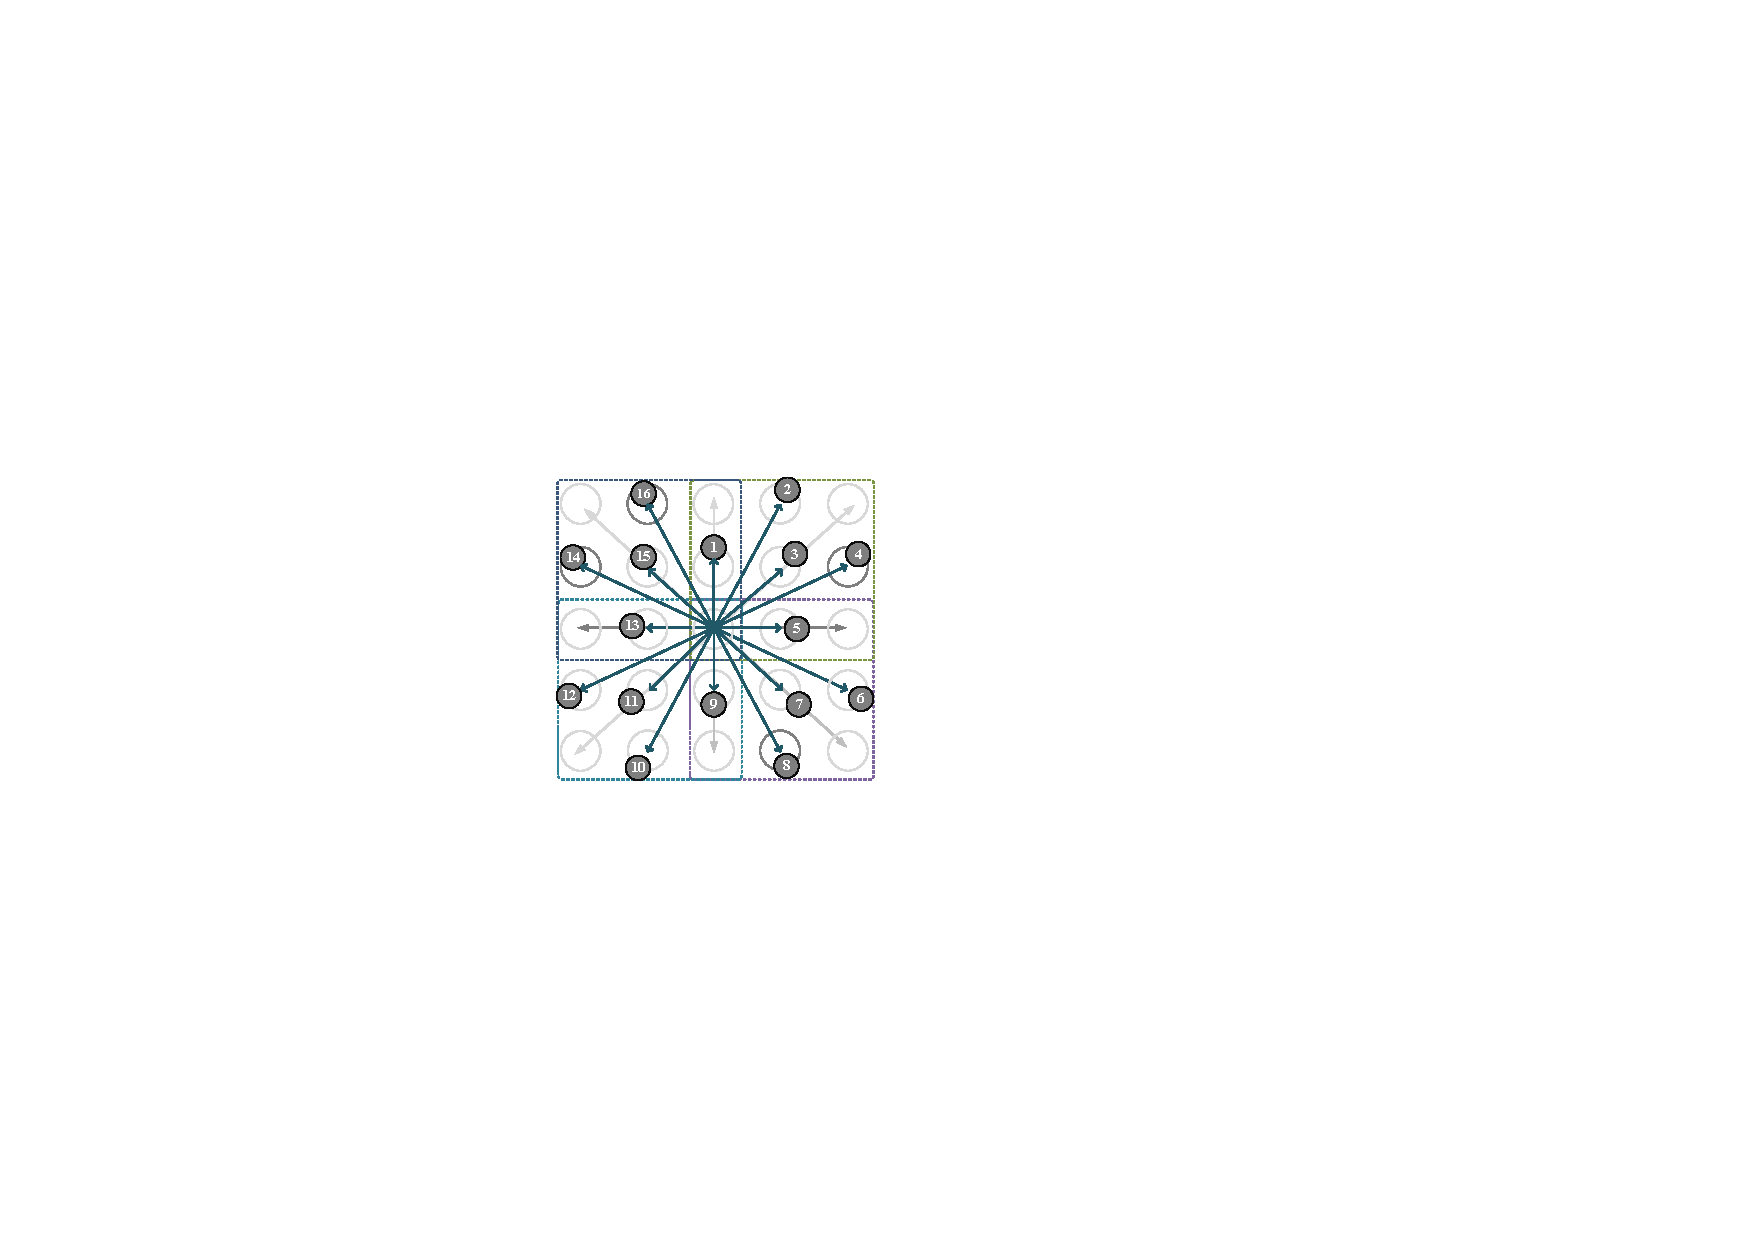
\includegraphics[width=\textwidth]{fig/7-1.pdf}\\
                \centering (a) line direction number
                \end{minipage}
            }
            \subfigure{
                \begin{minipage}[t]{0.25\textwidth}
                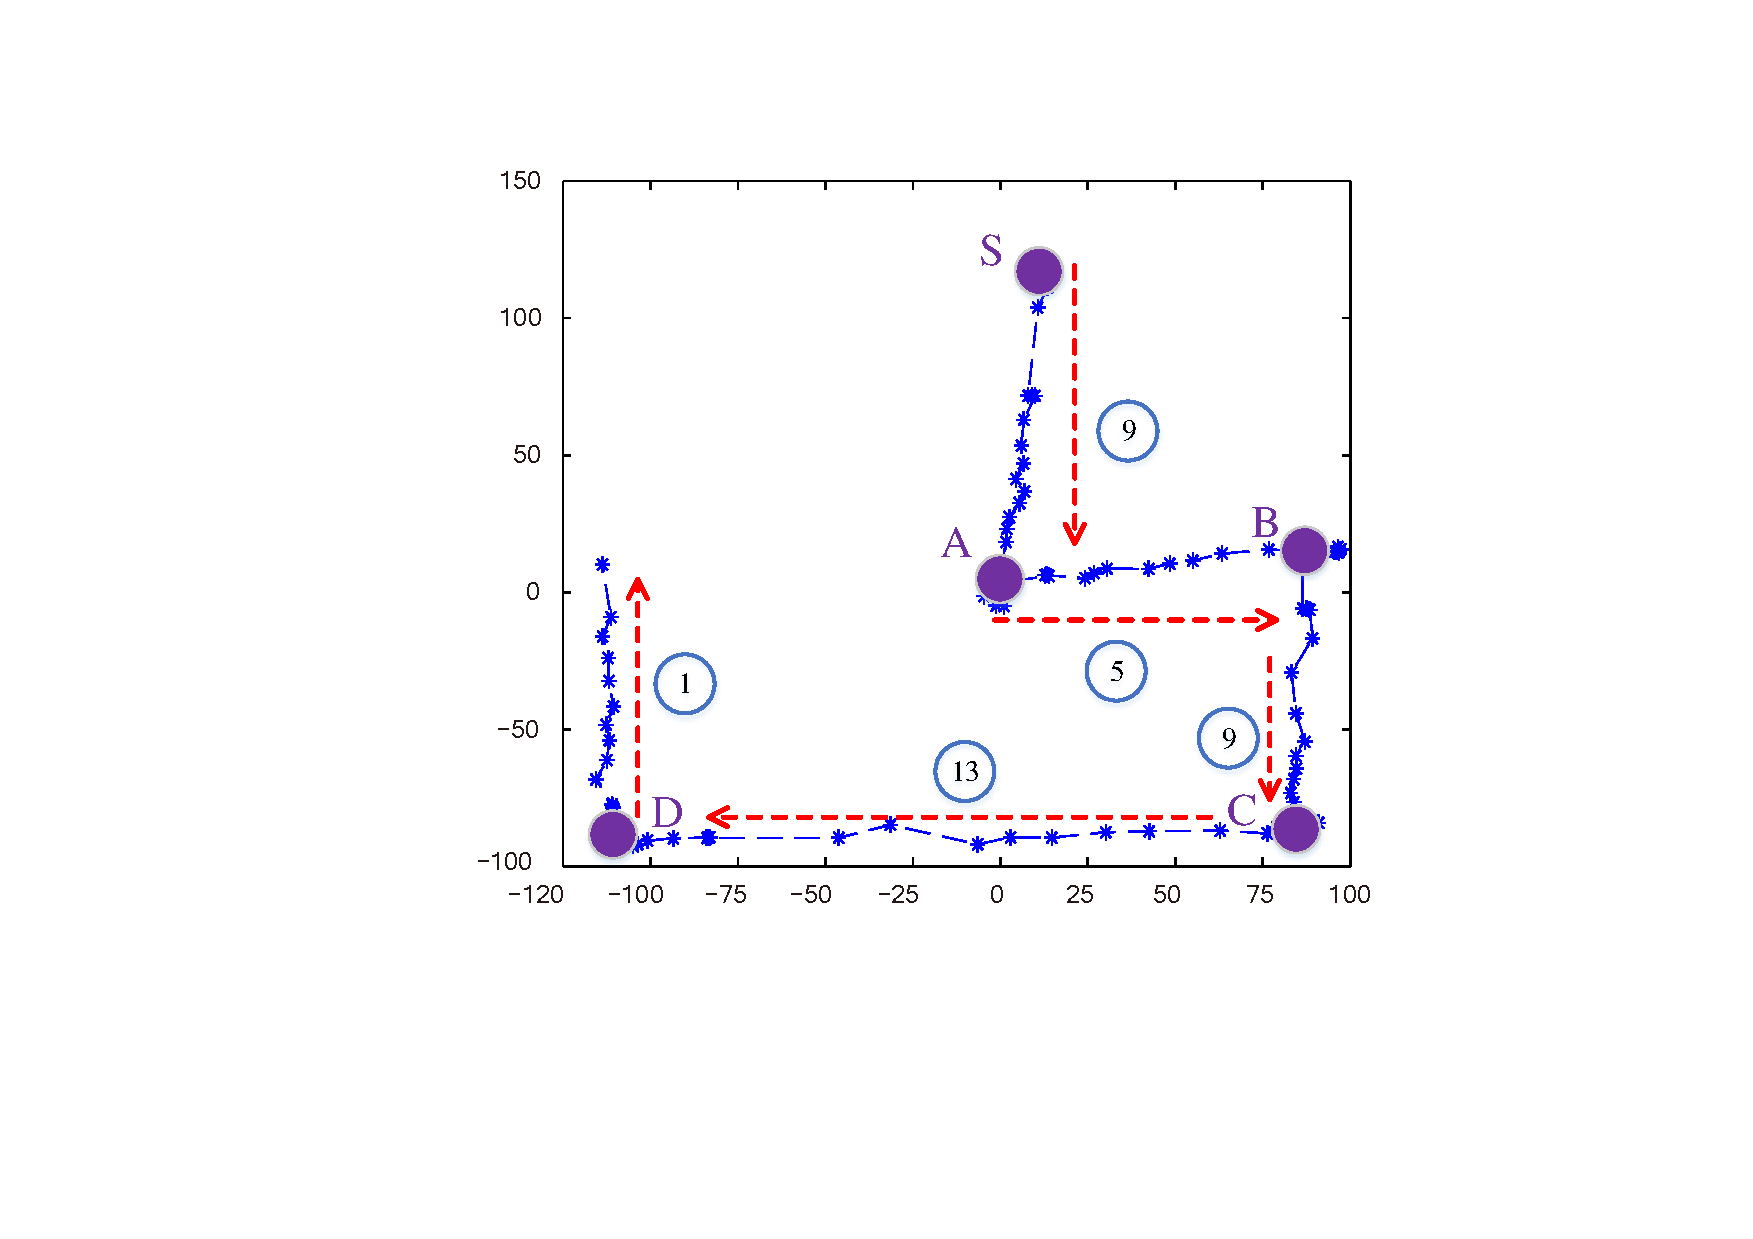
\includegraphics[width=\textwidth]{fig/7-2.pdf}\\
                \centering (b) numbering line segment of the tracked trajectory
                \end{minipage}
            }
            \caption{All possible line directions on a $3 \times 3$ Android pattern grid (a) and an example trajectory (b).}
            \label{fig:fig7}
            \vspace{-5mm}
        \end{figure}

        \begin{table}[t]
            \centering
            \caption{Mappings from line slopes and fingertip-horizontal movements to direction numbers}
            \label{tab:slopes}
            \small
            \begin{tabular}{lcccccccc}
                \toprule
                \textbf{Direction No.}& 1 & 2 & 3 & 4 & 5 & 6 & 7 & 8 \\
                \textbf{slope (L $\rightarrow$ R)} & $+\infty$ & $2$ & $1$ & $\frac{1}{2}$ & $0$ & $-\frac{1}{2}$ & $-1$ & $-2$ \\
                \midrule
                \textbf{Direction No.}& 9 & 10 & 11 & 12 & 13 & 14 & 15 & 16 \\
                \textbf{slope (R $\rightarrow$ L)} & $-\infty$ & $2$ & $1$ & $\frac{1}{2}$ & $0$ & $-\frac{1}{2}$ & $-1$ & $-2$ \\
                \bottomrule
            \end{tabular}
            \vspace{-5mm}
        \end{table}

       \noindent \textbf{Extract Direction Information.}
       In addition to the line length, we also want to know to which
       direction the finger moves. This information is useful for inferring which dots are selected to unlock the pattern.
       Figure~\ref{fig:fig7} (a) shows all possible 16
        directions on a $3 \times 3$ pattern grid. The
        directions are numbered from 1 to 16 in clockwise.
        For each line segment of the tracked trajectory, we calculate its line slope and the horizontal movement of the finger (i.e. left $\rightarrow$ right or vice versa).
        This information will then be checked against Table~\ref{tab:slopes} to determine the direction number of the line segment.
         The horizontal movement of the fingertip is determined by first using the temporal information to find out the start and the end points of the line and then comparing the horizontal coordinates of the two points.
        The line slope is also computed based on the coordinates of the
       start and the end points of the
        line segment.
        Figure~\ref{fig:fig7} (b) gives the direction number of each
        tracked line segment of a fingertip movement trajectory.

\begin{figure}[!t]
        \centering
        \subfigure{
            \begin{minipage}[b]{1.3cm}
            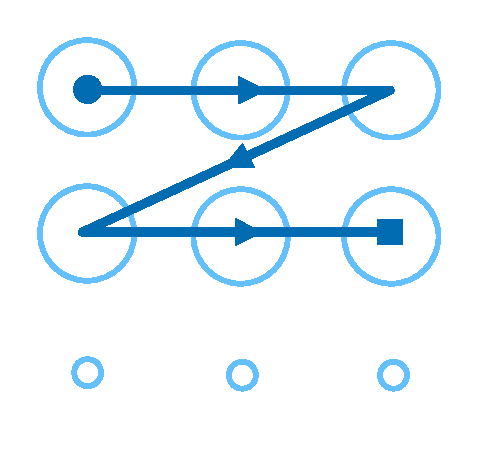
\includegraphics[width=1.3cm]{fig/600.pdf}\\
            \centering  a(1)
            \end{minipage}
        }
        \hspace{-0.2cm}
        \subfigure{
            \begin{minipage}[b]{1.3cm}
            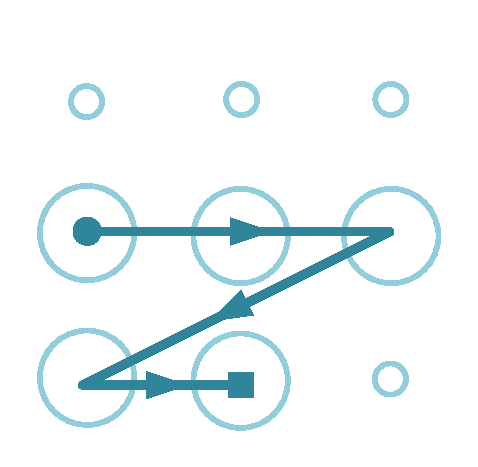
\includegraphics[width=1.3cm]{fig/601.pdf}\\
            \centering  a(2)
            \end{minipage}
        }
        \hspace{-0.2cm}
         \subfigure{
            \begin{minipage}[b]{1.3cm}
            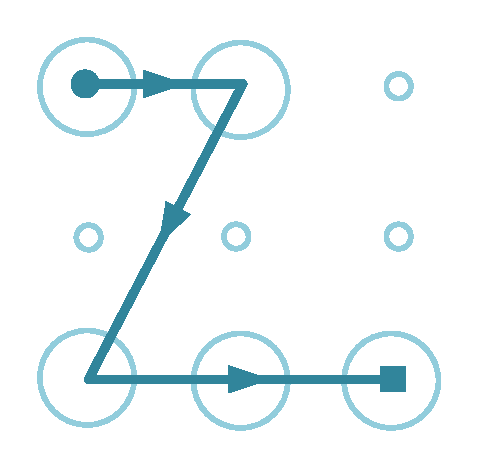
\includegraphics[width=1.3cm]{fig/602.pdf}\\
            \centering  a(3)
            \end{minipage}
        }
        \hspace{-0.2cm}
         \subfigure{
            \begin{minipage}[b]{1.3cm}
            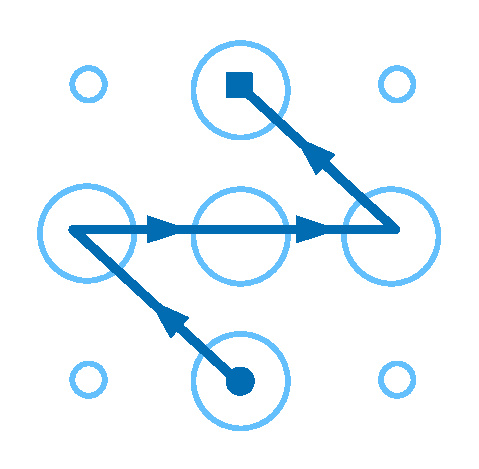
\includegraphics[width=1.3cm]{fig/603.pdf}\\
            \centering  a(4)
            \end{minipage}
        }
        \hspace{-0.2cm}
         \subfigure{
            \begin{minipage}[b]{1.3cm}
            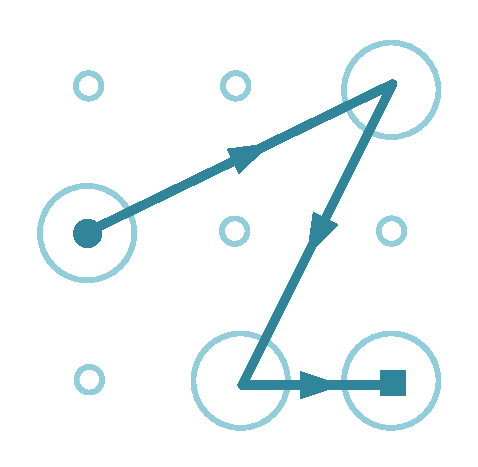
\includegraphics[width=1.3cm]{fig/604.pdf}\\
            \centering  a(5)
            \end{minipage}
        }
        \hspace{-0.2cm}
         \subfigure{
            \begin{minipage}[b]{1.3cm}
            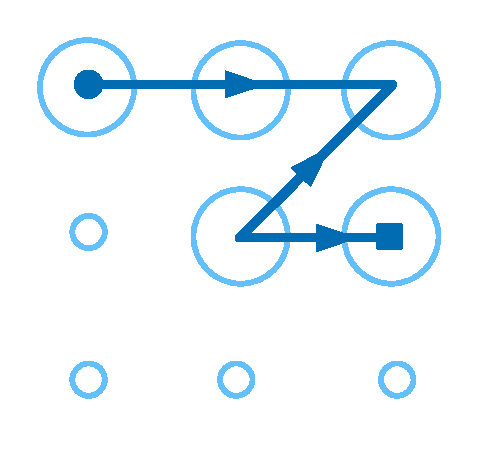
\includegraphics[width=1.3cm]{fig/605.pdf}\\
            \centering  b(1)
            \end{minipage}
        }
        \hspace{-0.2cm}
         \subfigure{
            \begin{minipage}[b]{1.3cm}
            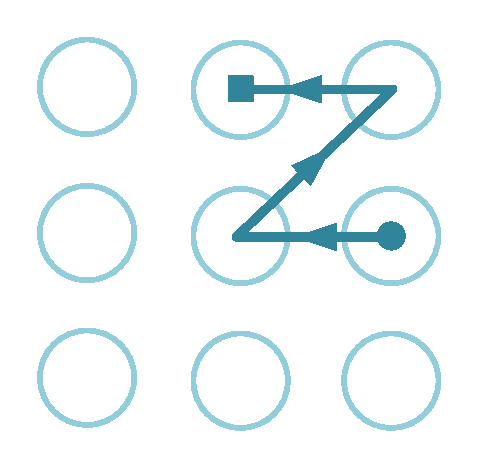
\includegraphics[width=1.3cm]{fig/606.pdf}\\
            \centering  b(2)
            \end{minipage}
        }
        \hspace{-0.2cm}
         \subfigure{
            \begin{minipage}[b]{1.3cm}
            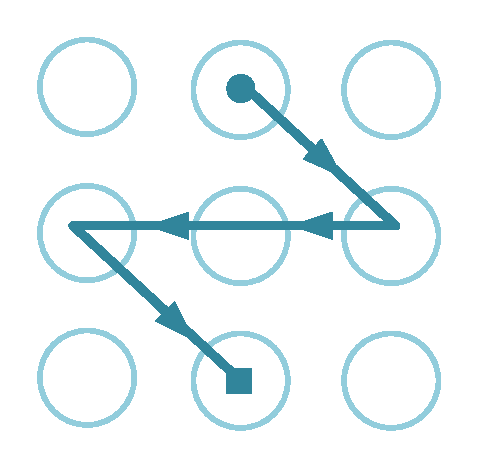
\includegraphics[width=1.3cm]{fig/607.pdf}\\
            \centering  b(3)
            \end{minipage}
        }
         \hspace{-0.2cm}
         \subfigure{
            \begin{minipage}[b]{1.3cm}
            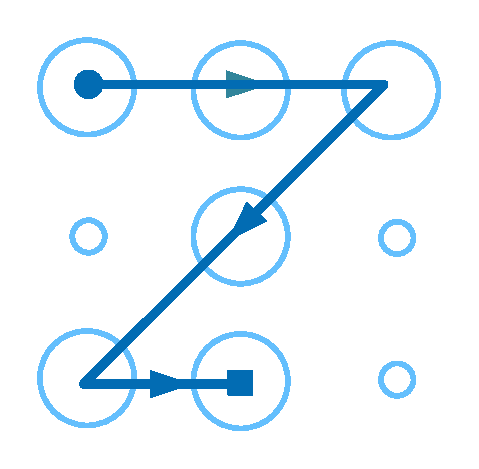
\includegraphics[width=1.3cm]{fig/608.pdf}\\
            \centering b(4)
            \end{minipage}
        }
         \hspace{-0.2cm}
         \subfigure{
            \begin{minipage}[b]{1.3cm}
            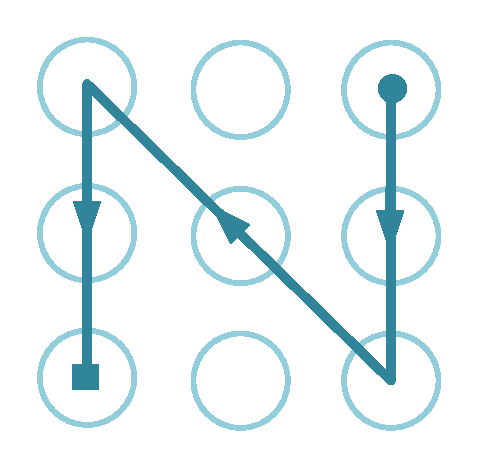
\includegraphics[width=1.3cm]{fig/609.pdf}\\
            \centering b(5)
            \end{minipage}
        }
         \hspace{-0.2cm}
         \subfigure{
            \begin{minipage}[b]{1.3cm}
            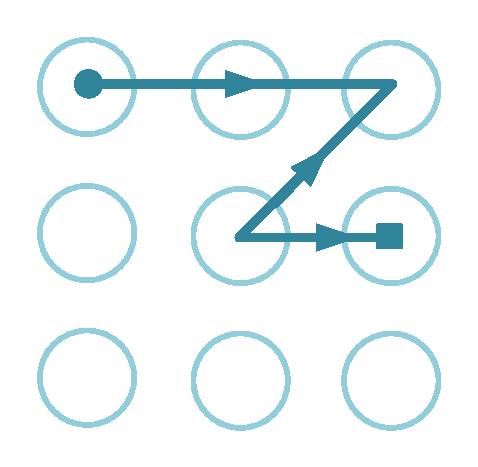
\includegraphics[width=1.3cm]{fig/610.pdf}\\
            \centering  c(1)
            \end{minipage}
        }
         \hspace{-0.2cm}
         \subfigure{
            \begin{minipage}[b]{1.3cm}
            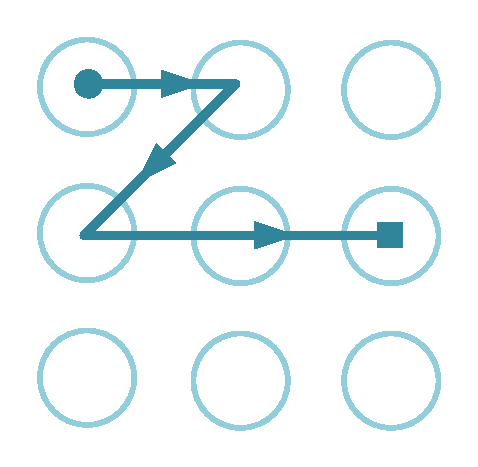
\includegraphics[width=1.3cm]{fig/611.pdf}\\
            \centering  c(2)
            \end{minipage}
        }
         \hspace{-0.2cm}
         \subfigure{
            \begin{minipage}[b]{1.3cm}
            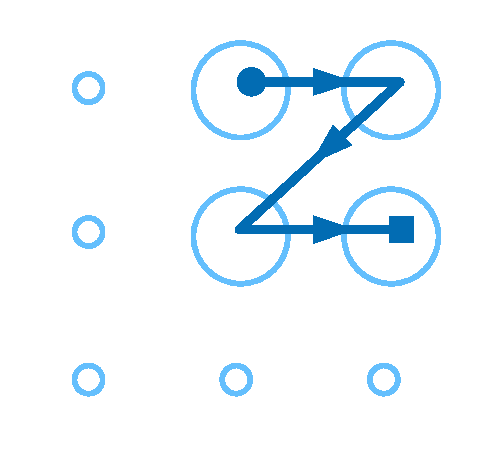
\includegraphics[width=1.3cm]{fig/612.pdf}\\
            \centering c(3)
            \end{minipage}
        }
         \hspace{-0.2cm}
         \subfigure{
            \begin{minipage}[b]{1.3cm}
            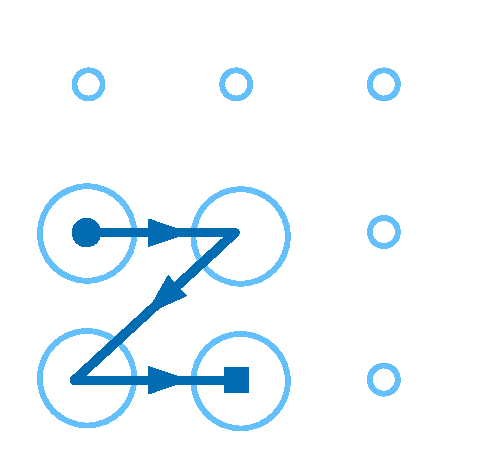
\includegraphics[width=1.3cm]{fig/613.pdf}\\
            \centering  c(4)
            \end{minipage}
        }
         \hspace{-0.2cm}
         \subfigure{
            \begin{minipage}[b]{1.3cm}
            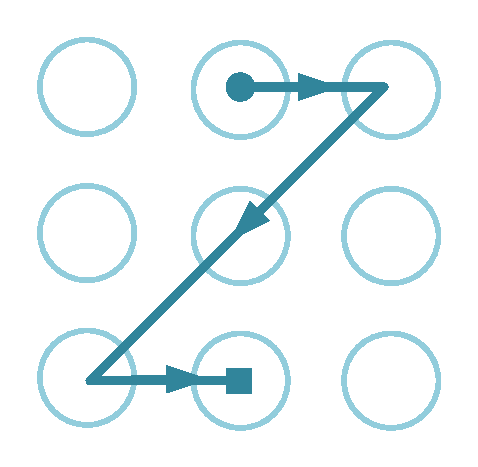
\includegraphics[width=1.3cm]{fig/614.pdf}\\
            \centering  c(5)
            \end{minipage}
        }
         \hspace{-0.2cm}
         \subfigure{
            \begin{minipage}[b]{1.3cm}
            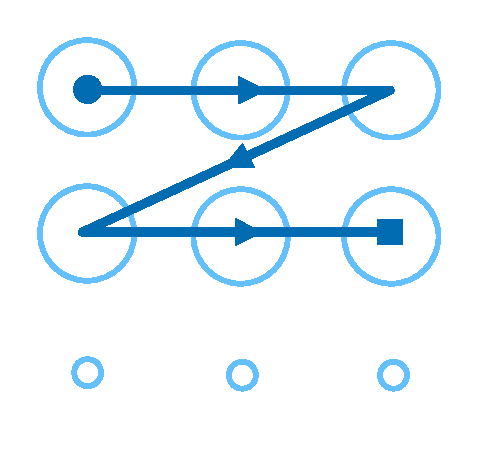
\includegraphics[width=1.3cm]{fig/615.pdf}\\
            \centering  d(1)
            \end{minipage}
        }
        \hspace{-0.2cm}
         \subfigure{
            \begin{minipage}[b]{1.3cm}
            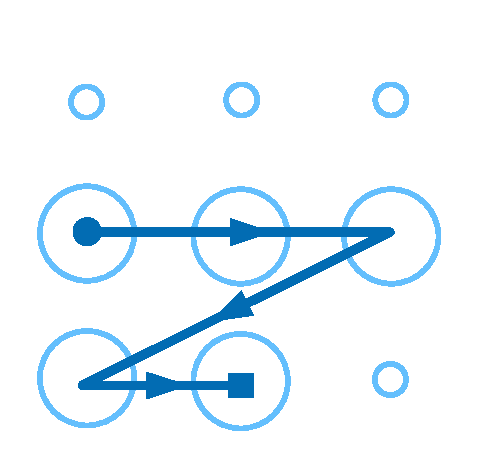
\includegraphics[width=1.3cm]{fig/616.pdf}\\
            \centering  d(2)
            \end{minipage}
        }
        \hspace{-0.2cm}
         \subfigure{
            \begin{minipage}[b]{1.3cm}
            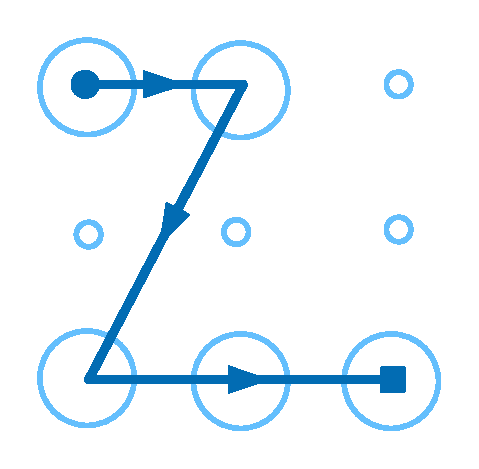
\includegraphics[width=1.3cm]{fig/617.pdf}\\
            \centering  d(3)
            \end{minipage}
        }
        \hspace{-0.2cm}
         \subfigure{
            \begin{minipage}[b]{1.3cm}
            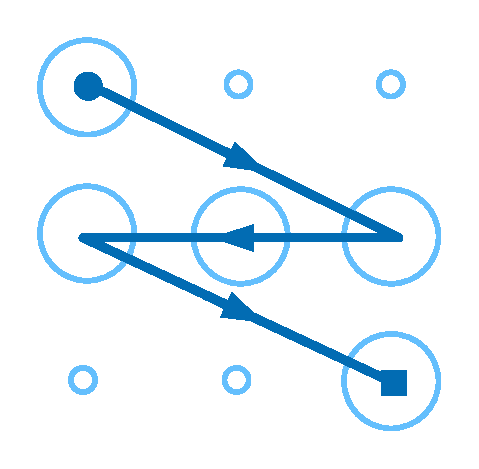
\includegraphics[width=1.3cm]{fig/618.pdf}\\
            \centering  d(4)
            \end{minipage}
        }
        \hspace{-0.2cm}
         \subfigure{
            \begin{minipage}[b]{1.3cm}
            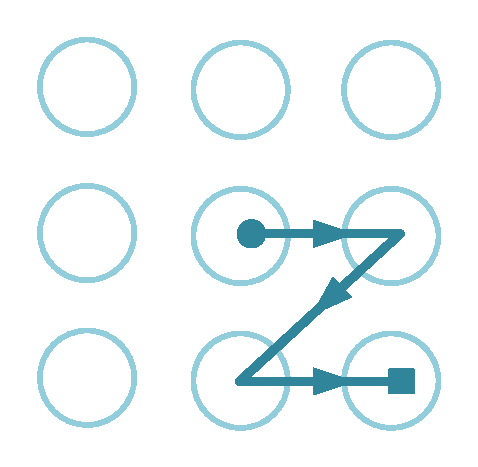
\includegraphics[width=1.3cm]{fig/619.pdf}\\
            \centering  d(5)
            \end{minipage}
        }
        \vspace{-2mm}
        \caption{Possible mappings for the tracked fingertip movement trajectory presented in Figure~\ref{fig:fig2} (d). }
        \vspace{-2mm}
        \label{fig:fig3}
        \vspace{-4mm}
    \end{figure}

%\begin{figure}[!t]
%    \centering
%    \subfigure{
%        \begin{minipage}[t]{0.11\textwidth}
%            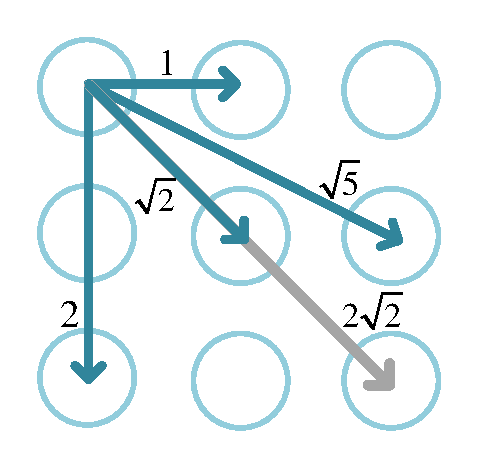
\includegraphics[width=\textwidth]{fig/physical_length.pdf}\\
%            \centering  (a) line length
%        \end{minipage}
%    }
%    \hspace{0.1cm}
%    \subfigure{
%        \begin{minipage}[t]{0.11\textwidth}
%            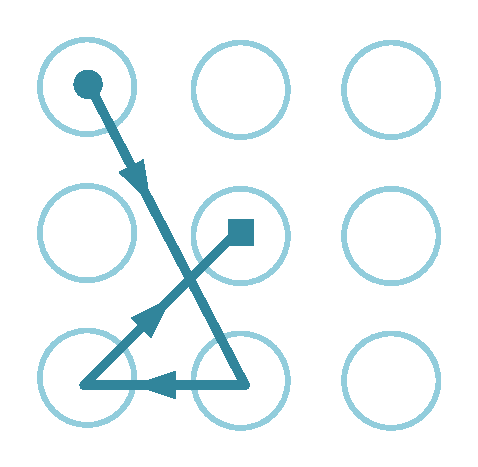
\includegraphics[width=\textwidth]{fig/intersection.pdf}\\
%            \centering  (b) line intersection
%        \end{minipage}
%    }
%    \hspace{0.1cm}
%    \subfigure{
%        \begin{minipage}[t]{0.11\textwidth}
%            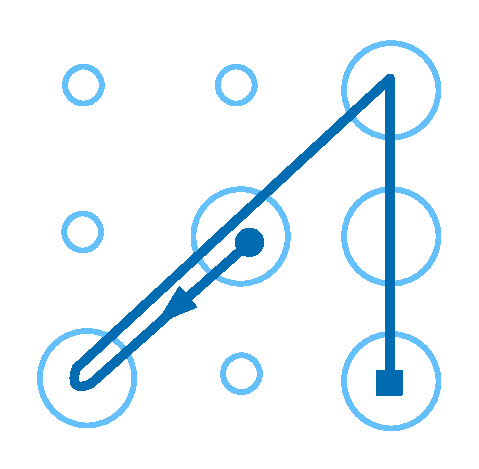
\includegraphics[width=\textwidth]{fig/overlap.pdf}\\
%            \centering  (c) overlapping lines
%        \end{minipage}
%    }
%    \caption{Illustrations of the terminologies used in Equation~\ref{equ:compscore}.}
%    \label{fig:intersection-overlap}
%    \vspace{-5mm}
%\end{figure}

    \subsubsection{Map the Tracked Trajectory to Candidate Patterns\label{section:identity}}
       In this step, we use the extracted geometry information to map the fingertip movement trajectory to a small number of candidate patterns which will then be ranked using a heuristic. %This process is described in Algorithm~\ref{alg:alg1}.

       \noindent \textbf{Identify Candidate Patterns.} Our implementation simply enumerates all possible
        patterns for a given pattern grid to identify candidate patterns, starting from the top-left touch point.
        We reject patterns that do not meet the requirements that the correct pattern is expected to have. The requirements are the number of line segments (this is checked by counting the number of turning points), and the length and the direction for each
        line segment.
        This is an \emph{automatic} process performed by our software system without any user involvement.
       We consider two line segments having the same length and slope if the difference between them is less
       than a threshold. Specifically, the relative length threshold, $lengthTh$, is set to 1.12 and the slope threshold, $directionTh$, is set to 0.25.
       %We chose these two values because they give the best performance in the experiments.
       To determine the thresholds, we have evaluated a range of possible values in our initial design experiments to choose the best performing values.

       \noindent \emph{Example:} We use the pattern depicted in Figure~\ref{fig:fig2} as an example to
       describe our algorithm. Figure~\ref{fig:fig3} gives several
       possible mappings for the fingertip movement trajectory shown in Figure~\ref{fig:fig2} (d). For this particular trajectory, the collections of lengths and directions are
       $L=\{l, \sqrt{2}l, l\}$ and $D=\{5, 11, 5\}$ respectively. Any pattern that does not meet $L$ or $D$ should not be considered as a candidate pattern for this trajectory.
       For this reason, Figure~\ref{fig:fig3} a(1)--a(5) will be rejected. Take Figure~\ref{fig:fig3} a(1) as an example,
       the line lengths and directions for all four line segments of this pattern are  $\{l,
       \frac{\sqrt{5}}{2}l, l\}$ and $\{5,12,5\}$ respectively. It does not meet the expected $L$ or $D$ and should be rejected.
       The patterns presented in b(1)--b(5) and c(1)--c(5) of Figure~\ref{fig:fig3}) will
       also be rejected for the same reason.

%\begin{figure}[!t]
%            \centering
%            \subfigure{
%                \begin{minipage}[b]{8cm}
%                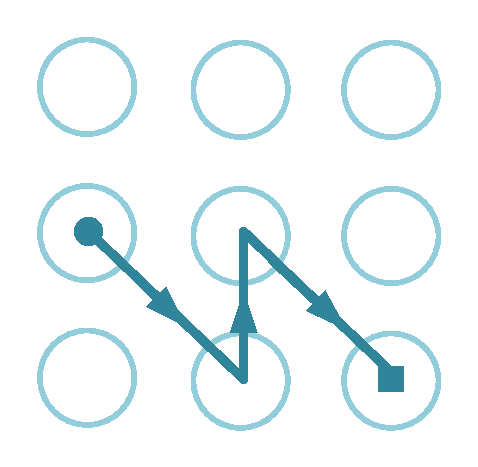
\includegraphics[width=1.3cm]{fig/9-1.pdf}
%                \hspace{0.1cm}
%                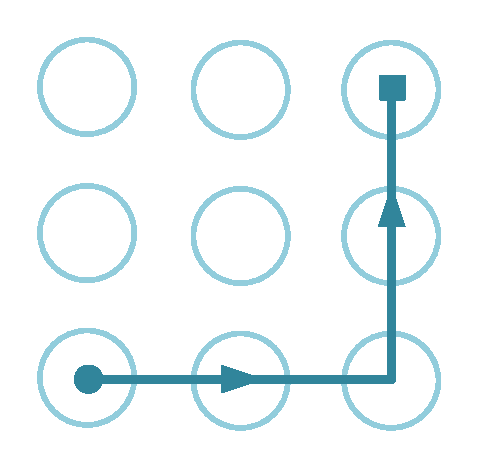
\includegraphics[width=1.3cm]{fig/9-2.pdf}
%                \hspace{0.1cm}
%                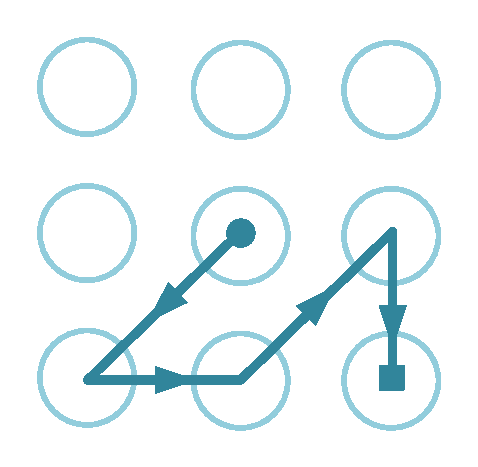
\includegraphics[width=1.3cm]{fig/9-3.pdf}
%                \hspace{0.1cm}
%                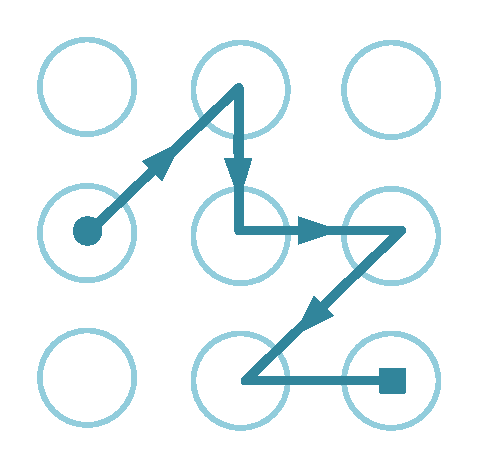
\includegraphics[width=1.3cm]{fig/9-4.pdf}
%                \hspace{0.1cm}
%                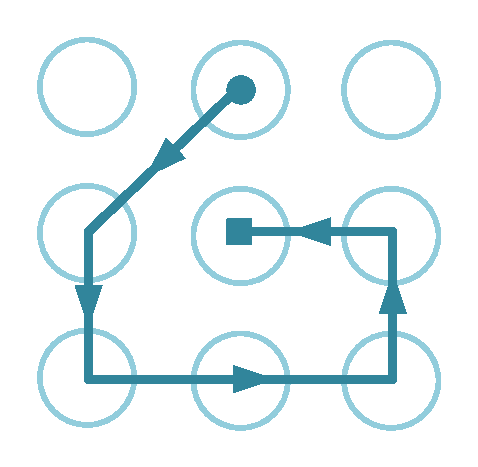
\includegraphics[width=1.3cm]{fig/9-5.pdf}\\
%                \centering  (a) Example patterns belong to the simple category.
%                \end{minipage}
%            }
%            \subfigure{
%                \begin{minipage}[b]{8cm}
%                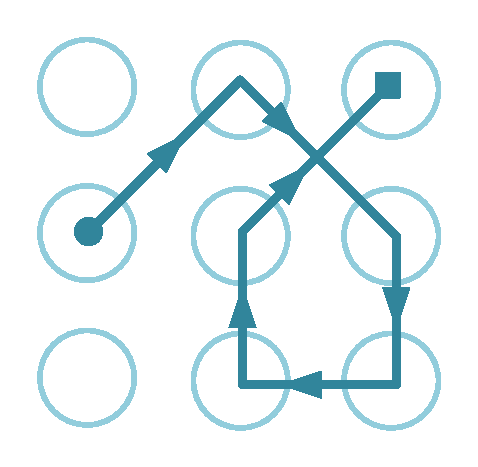
\includegraphics[width=1.3cm]{fig/9-6.pdf}
%                \hspace{0.1cm}
%                \includegraphics[width=1.3cm]{fig/9-7.pdf}
%                \hspace{0.1cm}
%                \includegraphics[width=1.3cm]{fig/9-8.pdf}
%                \hspace{0.1cm}
%                \includegraphics[width=1.3cm]{fig/9-9.pdf}
%                \hspace{0.1cm}
%                \includegraphics[width=1.3cm]{fig/9-10.pdf}\\
%                \centering  (b) Example patterns belong to the median category.
%                \end{minipage}
%            }
%            \subfigure{
%                \begin{minipage}[b]{8cm}
%                \includegraphics[width=1.3cm]{fig/9-11.pdf}
%                \hspace{0.1cm}
%                \includegraphics[width=1.3cm]{fig/9-12.pdf}
%                \hspace{0.1cm}
%                \includegraphics[width=1.3cm]{fig/9-13.pdf}
%                \hspace{0.1cm}
%                \includegraphics[width=1.3cm]{fig/9-14.pdf}
%                \hspace{0.1cm}
%                \includegraphics[width=1.3cm]{fig/9-15.pdf}\\
%                \centering  (c) Example patterns belong to the complex category.
%                \end{minipage}
%            }
%            \caption{Examples of patterns collected from our participants. Patterns are grouped into \emph{simple}, \emph{median} and \emph{complex} categories, according to their complexity scores. }
%            \label{fig:fig8}
%            \vspace{-3mm}
%        \end{figure}

       \noindent \textbf{Rank Patterns.} Candidates patterns are then ranked using a simple
        heuristic. The heuristic assumes a pattern starting from
        left dot of the grid is more likely to be the correct pattern over a
         pattern starting from a right dot. This assumption is supported
        by recent studies which show that people tend to select a left dot as the starting point
        to construct a pattern~\cite{uellenbeck2013quantifying,alpnorway}.
         If two candidate patterns
         start from the same dot, we consider the pattern with a
        longer total line length
        is more likely to be the correct pattern. Using these criteria,
        the five candidate patterns are ranked in order from subfigures d(1) to d(5) in
        Figure~\ref{fig:fig3}.
        %Therefore, an attacker would first try the candidate
%        pattern presented in Figure~\ref{fig:fig3} d(1).  This attempt will lead to a
%        successful attack for the example presented in Figure~\ref{fig:fig2}.
        Our experimental results show that
        this heuristic is effective.


